\documentclass[12pt] {book}
\usepackage[margin=1in]{geometry} %one inch margins
\renewcommand{\baselinestretch}{2} %double space, safe for fancy headers
\usepackage{setspace}
\usepackage{pslatex} %Times font
\usepackage{apacite} %apa citation style
\bibliographystyle{apacite}
%\usepackage[pdfborder={0 0 0}]{hyperref}%for hyperlinks without ugly boxes
\usepackage{graphicx} %for figures
\usepackage{enumerate} %for lists
\usepackage{booktabs}
%\usepackage{verbatim}
\usepackage[multiple, flushmargin]{footmisc} % 'multiple' to allow multiple footnotes separated by comma, 'flushmargin' to remove indentation of footnotes

\usepackage{amsmath}
\usepackage{amssymb}

\usepackage[svgnames]{xcolor} % Required to specify font color

\usepackage[document]{ragged2e} % left alignment (ragged right) instead of justified
\setlength{\RaggedRightParindent}{.5in} % 1/2 inch paragraph indentation
\usepackage{indentfirst} % indent first paragraphs after \section{} and friends

\usepackage{fancyhdr} %header
\pagestyle{fancy}
\fancyhf{}
\renewcommand{\headrulewidth}{0pt} % remove line at top of each page
\fancyfoot[R]{\thepage} % Set the right side of the footer to be the page number

% Redefine plain style, which is used for titlepage and chapter beginnings
% From http://tex.stackexchange.com/a/30230/828
\fancypagestyle{plain}{%
    \renewcommand{\headrulewidth}{0pt}%
    \fancyhf{}%
    \fancyfoot[R]{\thepage}%
}

\usepackage[font={small,sf},format=plain,labelfont=bf,up]{caption}


\DeclareMathOperator*{\argmax}{arg\,max}

%\setcounter{secnumdepth}{3} % numbers through \subsubsection
\setcounter{tocdepth}{3} % show numbers through \subsubsection in table of contents

\newcommand*{\titleGM}{\begingroup % Create the command for including the title page in the document
\hbox{ % Horizontal box
\hspace*{0.2\textwidth} % Whitespace to the left of the title page
\rule{1pt}{\textheight} % Vertical line
\hspace*{0.05\textwidth} % Whitespace between the vertical line and title page text
\parbox[b]{0.75\textwidth}{ % Paragraph box which restricts text to less than the width of the page

\singlespacing
{\noindent\Huge\bfseries Quantitative Methods \\ \noindent \LARGE for Historical Social Scientific Inquiry}\\[2\baselineskip] % Title
{\large \textit{with Bayesian Semiparametric \\ Structured Additive Regression Models}}\\[4\baselineskip] % Tagline or further description
{\Large \textsc{Jonah Sol Gabry}} % Author name

\textsc{Advisor: Gregory J. Wawro}

\vspace{0.5\textheight} % Whitespace between the title block and the publisher
{\noindent Quantitative Methods in the Social Sciences \\ \noindent Columbia University \\ \noindent New York, New York}\\[\baselineskip] % Publisher and logo
}}
\endgroup}

\begin{document}

\titleGM % This command includes the title page

\thispagestyle{empty}
{\singlespacing
\bigskip
\tableofcontents
}
\pagebreak
\setcounter{page}{1}

\chapter{Introduction}
\label{introduction}


Quantitative historical analyses in the social sciences should begin from the premise that 
parameters of interest may exhibit considerable variation over time. The entire enterprise 
makes little sense if it is assumed a priori that parameters will be constant -- parameter 
homogeneity should be discovered, not imposed. That is, there is a difference between 
hypothesizing that temporal variation in parameters is minimal and building a model that 
guarantees it. 
%Statistical modeling applied to the study of history is a double-edged sword. 
%It provides powerful techniques for learning from data, but also 

Nevertheless, there are many examples in the literature of statistical designs 
that presuppose parameters are invariant to time as well as models that do not explicitly 
make this assumption but lack the flexibility to discover variation if present.  Even methods that 
do attempt to allow for important variation often sacrifice some degree of statistical 
coherence, requiring other dubious assumptions or questionable treatment of the data.\footnote{
Part~\ref{cox_katz} of this thesis discusses one such example.}

\citeA{wawro_designing_2014} argue that the standard quantitative approaches for historical 
analysis in the social sciences are insufficient for addressing certain key features common to 
the most successful qualitative historical analyses. Citing the concerns of qualitatively-inclined 
political historians, Katznelson and Wawro contend that traditional methods lack attention to 
the nuanced ideas of temporality, periodicity, context and specificity.\footnote{Note that here 
periodicity is not used in the mathematical sense but rather refers how relationships between 
variables are influenced differently by break points in history at particular locations and times.}  
Rejecting ``... the idea that one must choose between historical depth and quantitative rigor," 
they propose an approach to historical social scientific inquiry that centers on relaxing structural 
assumptions and embracing parameter heterogeneity when appropriate (p. 527). Specifically, 
Wawro and Katznelson demonstrate that semi-parametric mixed models with historically relevant 
smoothing priors can accommodate greater parameter variation and let the data play a larger role 
in guiding inferences without sacrificing the stability of estimates as the parameters-to-data ratio 
becomes large.  

Wawro and Katznelson present these ideas in the context of the historical study of political 
institutions, and conduct reanalyses of two studies from the subfield of American Political 
Development. In this thesis, another empirical analysis is conducted demonstrating the merits 
of their recommendations. Similar in content and style to the applied statistics literature, 
considerable space is given to a formal description of the proposed statistical models and 
a discussion of estimation using the probabilistic programming 
language and Markov chain Monte Carlo sampler Stan, which is presented as an alternative to 
the computational strategy implemented by Katznelson and Wawro. It is argued that Stan can 
significantly contribute to the effort promoted by Wawro and Katznelson by enabling full Bayesian 
inference for a richer collection of statistical models than previously possible. 


%using Stan (which is not what K & W used) can significantly contribute to the effort they are promoting.  

%
%Many of the finer details of the statistical and computational methods (and challenges) involved in applying Katznelson and Wawro's recommendations are reviewed and then demonstrated in a reanalysis of . 
%\citeA{cox_gerrymandering_2007}
%ADD CLOSING SENTENCE





\chapter{Literature review}
\label{lit_review}

This chapter draws on the relevant statistical literature to review the theory behind the model applied in the empirical example in Chapter~\ref{cox_katz}. Section \ref{hierarchical} is a brief review of hierarchical models. Gaussian Markov random fields (GMRF) are defined and discussed in \ref{gmrf}. Finally, \ref{star} discusses Bayesian structured additive regression (STAR) models. 

\section{Hierarchical Bayesian models}
\label{hierarchical}

One of the many challenges of fitting models to data comprising multiple groups is confronting the tradeoff between bias and variance. An analysis that disregards between-group heterogeneity can yield parameter estimates with low variance but high bias. Group-by-group analyses, on the other hand, can reduce bias at the expense of high-variance estimates \shortcite{jackman_bayesian_2009}. While complete pooling or no pooling of data across groups is sometimes called for, nonhierarchical models for hierarchical data tend to underfit or overfit the data \shortcite{gelman_bayesian_2013}. Hierarchical modeling provides a compromise by allowing parameters to vary by group at lower levels of the hierarchical while estimating population-level parameters at higher levels. 

For example, consider a binomial model for the number of survey respondents $y$ in favor of a particular policy. It might be reasonable to estimate separate underlying levels of support $\theta$ for the policy for each of $R$ different geographical regions. However, it is also likely that there is some dependence between the $\theta$s that should be incorporated into the joint probability model. This can be expressed with a prior distribution for the $\theta$s conditional on shared hyperparameters $\phi$, potentially also estimating $\phi$ from the data 

\begin{align*}
y_r | \theta_r &\sim {\rm Bin}(N_r, \theta_r), \quad r = 1, \dots, R \\
\theta_r  | \phi &\sim p(\theta_r | \phi) \\
\phi & \sim p(\phi | \xi)  \\
\vdots
\end{align*}

In theory there is no limit to the number of levels in the hierarchy -- if the value of $\xi$ is not fixed in the example above then it too must be modeled -- however, in practice the data is informative only up to a point (and there are computational challenges to be considered as well). 

Perhaps the most important feature of hierarchical models is that inference for each group-level parameter is informed not only by the group-specific information contained in the data but also by the other groups as well \shortcite{jackman_bayesian_2009}.\footnote{The assumption of exchangeability is important here, but a sufficient discussion of exchangeability is beyond the scope of this thesis. See \citeA{gelman_bayesian_2013}.} This is commonly referred to as borrowing strength. In the example above, for instance, inferences about each $\theta_r$ are informed by $y_r$ but also by $y_{-r}$ through $\phi$.\footnote{The notation $y_{-r}$ is used here to refer to all $y$'s other than $y_r$ (e.g. $y_{-1} =  \{y_2, y_3, \dots, y_R\}$ ). Similar notation is used in later sections as well. } 

The term {\it hierarchical} is a suitable designation for a wide (theoretically unlimited) family of models, from the simple binomial example above to models with regressions at multiple levels. See \citeA{gelman_bayesian_2013} and \citeA{jackman_bayesian_2009} for more thorough and formal introductions to the topic.  




\section{Gaussian Markov random fields}
\label{gmrf}

The prior distributions of particular interest in this thesis are known as Gaussian Markov random field (GMRF) priors. The literature on GMRFs is vast, as they are frequently used in image processing and spatial statistics, however  GMRFs appear only rarely in quantitative social science and \citeA{wawro_designing_2014} is the first example extending the applications of GMRFs to historical social scientific inquiry. Before defining GMRFs it is first necessary to introduce some basic concepts from graph theory, particular the idea of an undirected graph. 

\subsection{Undirected graphs}
\label{undirected_graphs}

 \begin{figure}[htb]
\centering

\textsc{graph $\mathbf{A}$} \hspace{6cm} \textsc{graph $\mathbf{B}$} 

\vspace{.5cm}

\begin{tikzpicture}
\node[obs, fill=DarkSalmon] (r1) {$v_1$};
\node[obs, below left=of r1, fill=DarkSalmon] (r2) {$v_2$};
\node[obs, below=of r2, fill=DarkSalmon] (r3) {$v_3$};
\node[obs, below right=of r3, fill=DarkSalmon] (r4) {$v_4$};
\node[obs, above right=of r4, fill=DarkSalmon] (r5) {$v_5$};
\node[obs, above=of r5, fill=DarkSalmon] (r6) {$v_6$};
\edge [-, color=MidnightBlue, bend right=30] {r1} {r2} ;
\edge [-, color=MidnightBlue, bend left=30] {r1} {r6} ;
\edge [-, color=MidnightBlue] {r2} {r3} ;
\edge [-, color=MidnightBlue, bend right=30] {r3} {r4} ;
\edge [-, color=MidnightBlue, bend right=30] {r4} {r5} ;
\edge [-, color=MidnightBlue] {r5} {r6} ;
\end{tikzpicture}
%
 \hspace{4cm} 
 %
\begin{tikzpicture}
\node[obs, fill=SkyBlue] (r1) {$v_1$};
\node[obs, below right=of r1, fill=SkyBlue] (r2) {$v_2$};
\node[obs, below right=of r2,  fill=SkyBlue] (r3) {$v_3$};
\node[obs, below right=of r3,  fill=SkyBlue] (r4) {$v_4$};
\edge [-, color=DarkRed] {r1} {r2} ;
\edge [-, color=DarkRed, bend right=30] {r1} {r3} ;
\edge [-, color=DarkRed] {r2} {r3} ;
%\edge [-, color=DarkRed, bend left=30] {r2} {r4} ;
\edge [-, color=DarkRed] {r3} {r4} ;
\end{tikzpicture}
\vspace{.5cm}
\caption{Examples of simple undirected graphs. In \textsc{graph A} each node has two neighbors. In \textsc{graph B} node $v_4$ has only a single neighbor while the others each have two neighbors.}
\label{fig:undirected_graphs}
\end{figure}

 An undirected graph $\mathbf{G} = (V,E)$ is simply an ordered pair of sets containing the vertices (also called nodes) and edges of the graph, respectively. In what follows assume that $V$ and $E$ are finite and let $e_{ij} \in E$ denote the element in $E$ that corresponds to the edge connecting the vertices $v_i$ and $v_j$ in $V$. The term {\it undirected} refers to the fact that the edges lack orientation.\footnote{Intuitively, it is helpful to think of the edges of an undirected graph as line segments with no implied direction, whereas the edges in a directed graph can be thought of as arrows.} The {\it neighbors} of node $v_j$ are all nodes $v_i$ such that, for all $i \neq j$ , there is an edge $e_{ij}$. The notation $\partial^{\mathbf{G}}_j$ will be used for the {\it neighborhood} of node $v_j$ in graph  $\mathbf{G}$ and $\partial^\mathbf{G}$ for the set containing the neighborhoods for all nodes in $\mathbf{G}$.\footnote{$ \partial^\mathbf{G}_j = \{v_{i \neq j} \in V \,\vert\, e_{ij} \in E\}$ and $\partial^\mathbf{G} = \{\partial^\mathbf{G}_j \,\vert\, v_j \in V\}$.} For example, in Figure~\ref{fig:undirected_graphs}, $\partial^{\mathbf{A}}_1 = \{v_2, v_6\}$ and $\partial^{\mathbf{B}}_1 = \{v_2, v_3\}$.  For a more comprehensive discussion of undirected graphs in the context of GMRFs see \citeA{rue_gaussian_2005}. 
 

\subsection{GMRFs}
Let $\theta \in \mathbb{R}^D$ have a multivariate normal distribution with probability density function $p(\theta | \mu, \boldsymbol{\Sigma}) = \mathcal{N}_D (\theta | \mu, \boldsymbol{\Sigma})$. The random vector $\theta$ is said to form a GMRF with respect to the graph $\mathbf{G} = (V,E)$ if for each element in $\theta$ there is a corresponding node in $V$, and there is no edge $e_{ij}$ between nodes $v_i$ and $v_j$ \emph{if and only if} $\theta_i$ and $\theta_j$ are conditionally independent given all other elements of $\theta$ \shortcite{rue_gaussian_2005}.\footnote{$v_i \notin \partial^\mathbf{G}_{j} \iff \theta_i \bot \theta_j \mid \theta_{-ij}$}\footnote{This definition is consistent with the definition of Markov random fields in general. The random variables $\theta_1, \dots, \theta_D$ obey the requisite Markov properties describing pairwise, local, and global conditional independencies.} 

The relationship between $G$ and $\theta$ -- the information they provide about each other -- is fully contained in the covariance matrix $\boldsymbol{\Sigma}$, but it is not obvious from the individual elements of $\boldsymbol{\Sigma}$.\footnote{Nothing about the conditional independencies among the elements of $\theta$ can be inferred from the mean vector $\mu$.} It is more useful to instead consider the precision (inverse covariance) matrix $\mathbf{Q}=\boldsymbol{\Sigma}^{-1}$, for which it can be shown that conditional independence between $\theta_i$ and $\theta_j$ (no edge between nodes $v_i$ and $v_j$) always corresponds to a zero in cell $ij$ of the precision matrix, and vice-versa $(\forall i \neq j, \:\: v_i \in \partial_j \iff q_{ij} = 0)$.  For a simple proof see \citeA{rue_gaussian_2005}.\footnote{For intuition, the following interpretations of the elements of a precision matrix may also be helpful to keep in mind. For $i \neq j$ (the off-diagonal), $q_{ij}  = -Cov(\theta_i, \theta_j | \theta_{-ij}) $, the negative (flipped sign) covariance between $\theta_i$ and $\theta_j$ conditional on all $\theta$s except $i$ and $j$.  For $i = j$ (the diagonal),  $q_{ij} = Var(\theta_i | \theta_{-i})$, the variance of $\theta_i$ conditional all the variables except $\theta_i$.}






\section{Bayesian STAR models}
\label{star}

An extension of generalized linear models (GLMs), semiparametric structured additive regression (STAR) models replace the linear predictor with a structured additive predictor of the form
%
\begin{equation*}
\eta =  u'\gamma + \sum_{j} f_j (x_j) =  u'\gamma + f_1(x_1) + \ldots + f_j(x_j) + \ldots + f_J(x_J),
\end{equation*}
%
\noindent which can include nonlinear unknown functions of covariates as well as linear components \shortcite{fahrmeir_bayesian_2001}. 

From the Bayesian perspective, the non-varying parameters $\gamma$ as well as the unknown functions $f_1, \dots, f_J$ are treated as random variables distributed according to priors that we must specify. For an unknown function $f_j$ of a covariate $x_j$ let $\mathbf{f}_j^{eval}$ denote the vector of function evaluations of $f_j$ at each of the $N$ observed values of $x_j$ 

\begin{equation*}
\mathbf{f}_j^{eval} = \left(f_j(x_{1j}), \dots f_j(x_{Nj})\right)'.  
 \end{equation*}
 
\noindent Then $\mathbf{f}_j^{eval}$ is treated as a random vector, which, following \citeA{brezger_generalized_2006}, can conveniently be expressed as the matrix product $\mathbf{M}_j \theta_j$ of a design matrix $\mathbf{M}_j$ and a parameter vector $\theta_j$. GMRF priors for each parameter vector $\theta_j$ take the general form

\begin{equation*}
p(\theta_j | \tau^2_j) 
\propto 
\frac{1}{\left(\tau^2_j\right)^{{\rm rank}(\mathbf{P})/2} }
\exp{\left\{-\frac{1}{2\tau^2_j} \theta_j' \mathbf{P} \theta_j\right\}}
\end{equation*}

\noindent where $\mathbf{P}$ is a penalty matrix whereby we operationalize our prior assumptions about the smoothness of the unknown function $f_j$. 

To provide some intuition, suppose we are interested in learning about an effect with assumed variation over geographic regions.  A simple map with $R$ distinct regions $r_1, r_2, \dots r_R$ can be represented as undirected graph $G$ with vertices $V = \{1, 2, \dots, R\}$ and edges $E$ connecting vertices corresponding to neighboring (or proximate) regions. Assuming some degree of dependence of the quantity of interest across regions, a prior on a parameter vector $\theta = (\theta_1, \dots, \theta_r)$ can be constructed such that the matrix $\mathbf{P}$ has a zero in the $ij$th cell if and only if $\theta_i$ and $\theta_j$ (the parameters corresponding to regions $r_i$ and $r_j$) are assumed to be independent conditional on $\theta_{-ij}$. Then $\theta$ is a GMRF with respect to $G$ with $\boldsymbol{\Sigma}^{-1} = \mathbf{Q} = \mathbf{P}/\tau^2$. 

\subsection{The penalty matrix} 
\label{penalty_matrix}

More specifically, the penalty matrix $\mathbf{P}$ can be constructed as  $\mathbf{P} = \mathbf{D} - \mathbf{A}$, where $\mathbf{A}$ is a symmetric matrix with $a_{ij} = 1$ if temporal or spatial units $i$ and $j$ are considered neighbors (the associated graph $G$ has an edge between nodes $i$ and $j$) and 0 otherwise, and $\mathbf{D}$ is a diagonal matrix such that $\forall i = j, \: d_{ij} = \sum_j a_{ij}$. The matrices $\mathbf{A}$ and $\mathbf{D}$ are commonly referred to as the adjacency and degree matrices because encoded in $\mathbf{A}$ are all neighbor relationships (temporal or spatial) and the (diagonal) elements of $\mathbf{D}$ are equal to the number of neighbors (the degree) of each vertex in the graph $G$. 

To illustrate why this form of $\mathbf{P}$ captures these particular assumptions, consider $N$ measurements of a variable $x$, with each measurement of $x$ made at one of $T$ evenly spaced points in time. For simplicity, but without loss of generality,  assume that $x$ is a unit of time and there is exactly one measurement per time period.  The sequence $(x^{[t]})_{t=1}^T$ then corresponds to a grid of points on a line.  \citeA{fahrmeir_bayesian_2001} suggest several possible choices for a prior on a smooth function $f(x)$, the simplest of which is a first order random walk ($RW_1$) prior.  Under the $RW_1$ prior, the first differences $\Delta_t = f(x^{[t]}) - f(x^{[t-1]})$ are treated as independent and identically distributed standard normal random variables. 

While this formulation of the $RW_1$ prior is {\it directed}, conditioning also on $f(x^{[t+1]})$ -- one step into the future -- forms an undirected $RW_1$, where the neighbors of time $t$ are both $t-1$ and $t+1$.  The associated graph $G$ therefore has vertices $V=\{v_t : t=1,\dots,T\}$, each of which has two neighbors, with the exception of $v_1$ and $v_T$, which have one neighbor. The penalty matrix $\mathbf{P}$ corresponding to the $RW_1$ prior with equally spaced observations is the tridiagonal matrix

\begin{equation*}
\mathbf{P} = 
\begin{bmatrix}
1  	& -1 	& 		& 	& \\
-1  	& 2 	& -1 		& 	& \\
  	& -1 	& \ddots 	& \ddots	& \\
  	&  	& \ddots 	& 2 	& -1\\
  	&  	& 		& -1 	& 1\\
\end{bmatrix}
\end{equation*}

\noindent which can be derived by computing the difference of the appropriate degree and adjacency matrices \shortcite{brezger_generalized_2006}.\footnote{The construction of $\mathbf{P}$ as the matrix difference $\mathbf{D} - \mathbf{A}$ also allows for the estimation of a parameter $\omega \in [0,1]$, which, as a coefficient on $\mathbf{A}$, can be interpreted as representing the strength of spatial or temporal dependence \shortcite{rue_gaussian_2005}. The resulting precision matrix $\mathbf{Q}= (\mathbf{D} - \omega \mathbf{A})/\tau^2$ is the defining feature of the conditional autoregressive (CAR) model.  When $\omega = 1$, and thus $\mathbf{P}= \mathbf{D} - \mathbf{A}$, the model is sometimes referred to as an intrinsic CAR model.
} The $RW_1$  can be extended to an $RW_2$ prior by also considering the measurements $x^{[t-2]}$  and $x^{[t+2]}$ to be neighbors of $x^{[t]}$. 


\subsection{Hyperpriors}
\label{hyperpriors}

To complete the hierarchical model requires also specifying hyperpriors $p(\tau_j^2)$.  Assigning a prior distribution to the variance hyperparameter $\tau_j^2$ allows for the simultaneous estimation of a smoothing function $f_j$ and the amount of smoothness. \citeA{fahrmeir_bayesian_2001} and \citeA{brezger_bayesx:_2005} recommend a weakly informative but proper inverse-gamma prior on $\tau_j^2$. However, in light of concerns about this type of inverse-gamma prior raised by \citeA{gelman_prior_2006}, in this thesis several priors for $\tau^2_j$ are used and compared to check the degree to which the results are sensitive to the choice of prior.




%Cox and Katz (2007) is a study of bias and responsiveness in the 46th through 106th Congresses. Cox and Katz are predominantly concerned with estimating the parameters $\lambda = \{\lambda_t : t = 46, \dots, 106\}$ representing bias in each $C_t$ (Congress t), which they do by maximum likelihood estimation of grouped logit models with linear predictor
%
%$$ \lambda_t + \rho_t \log{\left(\frac{v_t}{1 - v_t} \right)}, $$
%
%\noindent where $\rho$ is responsiveness and $v$ is average Democratic vote share. They use this strategy to estimate what they call ``a sort of running average" of the bias across time, where they take as their estimate of $\lambda_t$ the average estimate of $\lambda$ over the seven congresses centered at $t$, i.e., the set of congresses $\{C_\tau, t-3 \leq \tau \leq t+3\}$. 
%
%Note that this strategy requires using the data for each Congress up to seven times, which can lead to overly precise parameter estimates. Moreover, the estimation strategy used by Cox and Katz treats each of the seven congresses centered at $t$ as providing {\it equal} information about $\lambda_t$, which is unlikely to be the case. 
%
%Many new possibilities are available to us if we can reformulate their model according to the Bayesian approach advocated above. Let $x = \log{\left(\frac{v_t}{1 - v_t} \right)}$. We use the addititive predictor
%
%$$ \eta = f_1(\lambda) + f_2(x),$$
%
%where the $f_j$ are unknown functions such that the vector of evaluations of $f_j$ can be expressed as the product $\theta_j \mathbf{M}_j$ of a parameter vector $\theta_j$ and a design matrix $\mathbf{M}_j$.  We can then assign a prior for $f_j$ by specifying a suitable $\mathbf{M}_j$ and a (typically partially improper) multivariate normal prior 
%%
%$$ p(\theta_j | \tau_j^2) \propto \exp{\left(-\frac{1}{2\tau_j^2} \theta_j^T \mathbf{P}^{-1} \theta_j \right)}, $$
%
%\noindent where we choose to specify a penalty matrix $\mathbf{P}$ that represents our assumptions of temporal dependence between adjacent Congresses. 
%
% For example, suppose we want to specify a prior that reflects a belief that $\partial_t = \{C_{t-2}, C_{t-1}, C_{t+1}, C_{t + 2} \}$ provides information about $C_t$. We will refer to the elements of $\partial_t$ as the {\it neighbors} of $C_t$. We can use an undirected form of a second order random walk or autoregressive prior to penalize deviations from this hypothesized trend, which corresponds to setting $\mathbf{P} = \mathbf{D} - \mathbf{A}$, where $\mathbf{A}$ is a symmetric matrix with $a_{ij} = 1$ if $C_j \in \partial_i$ and 0 otherwise, and $\mathbf{D}$ is a diagonal matrix such that $\forall i = j, \: d_{ij} = \sum_j a_{ij}$.\footnote{It can be useful to conceptualize the neighbor relations as an undirected graph $G$ with vertices $V= \{C_t, t = 46, \dots, 106\}$ and edges connecting the vertices corresponding to neighboring congresses. The penalty matrix $\mathbf{P}$ then has a zero for each missing edge and the resulting multivariate normal distribution is said to form a Markov random field with respect to $G$. The matrices $\mathbf{A}$ and $\mathbf{D}$ are commonly referred to as the adjacency and degree matrices.}   We then specify a hyperprior $p(\tau^2)$, completing the hierarchical model and enabling the concurrent estimation of the unknown function $f$ and the amount of nonparametric smoothing (Fahrmeir and Lang, 2000). 
% 
% Note that this approach enables us to account for temporal dependence without reusing the data to estimate separate a model for each congress. The Bayesian approach advocated here allows the specification of more intricate temporal relationships that better reflect our assumptions of association across time (and across space in other contexts). For example, a second order random walk prior treats $C_{t-1}$ and $C_{t+1}$ as being more informative than $C_{t-2}$ and $C_{t+2}$ about bias in $C_t$, which seems more reasonable. 


\chapter{Empirical example: Cox and Katz (2007)}
\label{cox_katz}

To demonstrate the benefits of the methods proposed by \citeA{wawro_designing_2014}, we conduct a reanalysis of \citeA{cox_gerrymandering_2007}, a study of bias and responsiveness in congressional roll-call votes in the 46th through 106th US Congresses. Cox and Katz's findings suggest persistent bias towards the majority party with particularly elevated levels during the periods from 1889-1910 and 1961-2000, known as the period of ``czar rule" and the post-packing era, respectively. Analyzing the data using Bayesian STAR models we find much weaker evidence for bias towards the majority over the time periods in question. 

\section{Definitions}


\paragraph{Bias}
In the legislative context of Cox and Katz's analysis, bias is defined as an advantage for one party in the efficiency with which its votes translate into legislative victories. For example, consider a majority party with only a small advantage in the number of seats its members occupy. If the majority is well-organized and unified it may win a much larger proportion of votes than its slim seat advantage would typically suggest. 

\paragraph{Responsiveness} MISSING DEFINITION


\section{Data}

The data include -- with a few exceptions detailed below -- all roll-call votes in the U.S. House of Representatives during the 46th through 106th Congresses, corresponding to the period from 1879 to 2001.  Following Cox and Katz, excluded from the analysis are any records that meet at least one of the following three conditions:

\begin{itemize}
\singlespacing
\item The majority of both parties voted for the same position 
\item The purpose of the vote was electing the Speaker of the House
\item The vote required a two-thirds majority for passage.
\end{itemize}

The resulting data consist only of votes that required a simple majority for passage and on which the Republican and Democratic parties were in clear opposition. 

Let $RC_{it}$ denote the result of roll-call vote $i$ in Congress $t$ such that 

{\singlespacing
$$ RC_{it} =
\begin{cases} 
1, & \text{ if Democratic position wins vote $i$ in Congress $t$} \\
0, & \text{ if Republican position wins vote $i$ in Congress $t$.}
\end{cases}
$$
}
%
Here, the Democratic position refers to the outcome preferred by the majority of Democrats.  The definition is analogous for the Republican position.

%The outcomes of interest are the number of wins ($w_t^{DEM}$) and proportion of wins ($p_t^{DEM}$) for the Democratic position in each Congress $t$
%
%$$ w_t^{DEM} = \sum_{i=1}^{n_t} RC_{it}, \qquad p_t^{DEM} = w_t^{DEM} / n_t.\footnote{The superscript {\it MAJ} (e.g. $w_t^{MAJ}$) will be used later in the thesis as a general way of referring to the majority party in a specific time period. While the data is organized and more naturally described in terms of $w_t^{DEM}$ and $w_t^{REP}$ (which is just $n_t-w_t^{DEM}$), the proposed statistical model is more straightforward to implement in terms of $w_t^{MAJ.}$}$$
%
%Here $n_t$ is the number of roll-call votes in Congress $t$, which ranges from a minimum of 33 votes in the 70th Congress (1927-1929) to a maximum of 836 votes in the 104th Congress (1995-1997). The median number is 143 votes.  
%
%
%The sole predictor of interest is $v^{RATIO}$, the ratio of the average vote share earned by the Democratic position to the average vote share earned by the Republican position in each Congress.  For each Congress the average is taken over all roll-call votes.  For vote $i$ in Congress $t$, let $\pi_{it}^{DEM}$ be the proportion of representatives who cast their vote in favor of the Democratic position.  Then the mean vote shares for the Democratic and Republican positions in Congress t is
%
%{\singlespacing
%$$v_t^{DEM} = \frac{1}{n_t} \sum_{i=1}^{n_t} \pi_{it}^{DEM}, \qquad v_t^{REP} = 1 - v_t^{DEM}$$
%}
%%
%\noindent and the ratio of Democratic to Republican vote shares is simply $v_t^{RATIO} = v_t^{DEM} / v_t^{REP}$. Figure~\ref{fig:log_vratio_vs_ptdem} shows $\log{(v^{RATIO} )}$ plotted against $p^{DEM}$. The shape of the curve is similar to the standard seats-votes curve used in analyses of bias and responsiveness in electoral contexts. The curve is analogous in the legislative context of Cox and Katz's example, although we are not concerned with seat shares in a given Congress but rather roll-call vote shares ($p_t^{DEM}$ and $p_t^{REP}$). This is discussed further in the Methods section. 
%
%The trends of $\log{(v^{RATIO} )}$ and $p^{DEM}$ over time are shown in the visual summary of the data set in Figure~\ref{fig:data_summary}.
%
%%FIGURE
%\begin{figure}
%\centering
%	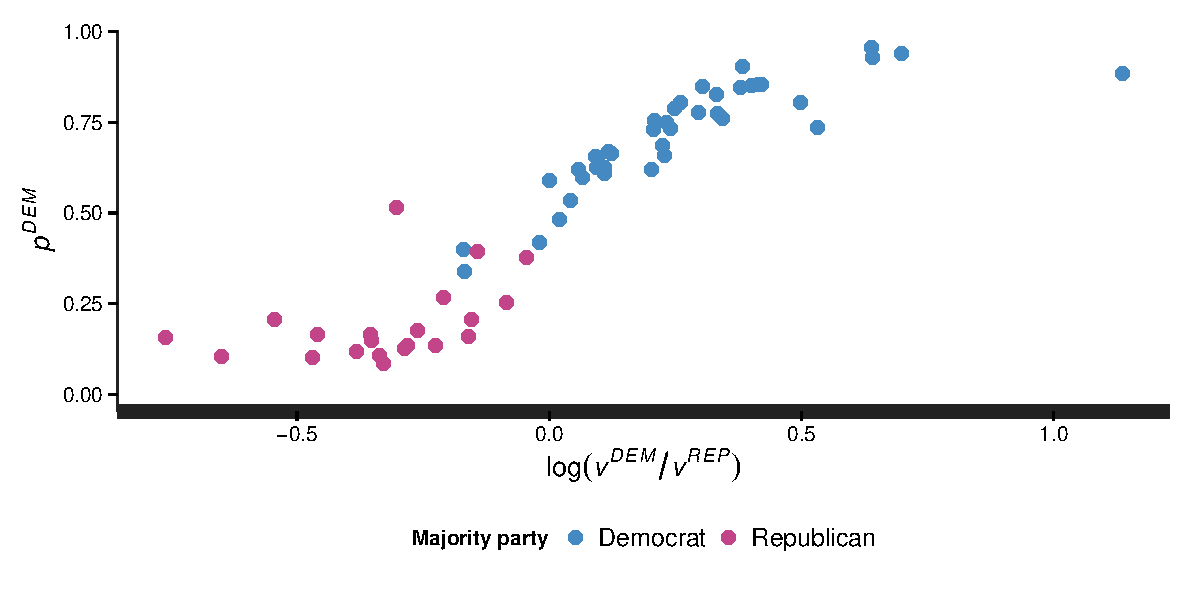
\includegraphics[scale=0.75]{sections/figs/logvratio_vs_pdem}
%\caption{$\log{(v^{RATIO} )}$  vs. $p^{DEM}$}
%\label{fig:log_vratio_vs_ptdem}
%\end{figure}
%%
%



The outcomes of interest are the number of wins ($w_t^{MAJ}$) and proportion of wins ($p_t^{MAJ}$) for the majority party position in each Congress $t$. Let $n_t$ denote the number of roll-call votes in Congress $t$.\footnote{In the data $n_t$ ranges from a minimum of 33 votes in the 70th Congress (1927-1929) to a maximum of 836 votes in the 104th Congress (1995-1997). The median number is 143 votes.}  Then

$$w_t^{MAJ} =
\begin{cases} \sum_{i=1}^{n_t} RC_{it}, & \text{ if Democrats hold majority} \\
n_t - \sum_{i=1}^{n_t} RC_{it}, & \text{ if Republicans hold majority} \\
\end{cases}
 $$
 
\noindent and $p_t^{MAJ} = w_t^{MAJ} / n_t$.

The sole predictor of interest is $v^{RATIO}$, the ratio of the average vote share earned by the majority party position to the average vote share earned by the minority party position in each Congress.  For each Congress the average is taken over all roll-call votes.  For vote $i$ in Congress $t$, let $\pi_{it}^{DEM}$ be the proportion of representatives who cast their vote in favor of the Democratic position.  Then the mean vote shares for the Democratic and Republican positions in Congress t are

{\singlespacing
$$v_t^{DEM} = \frac{1}{n_t} \sum_{i=1}^{n_t} \pi_{it}^{DEM}, \qquad v_t^{REP} = 1 - v_t^{DEM},$$
}
%
\noindent and the ratio of Democratic to Republican vote shares is simply $v_t^{DEM} / v_t^{REP}$. The notation $v^{RATIO}$ will be used as shorthand for the ratio $v_t^{MAJ} / v_t^{MIN}$, that is 

$$ v^{RATIO} = 
\begin{cases} 
v_t^{DEM} / v_t^{REP}, & \text{ if Democrats hold the majority,} \\
v_t^{REP} / v_t^{DEM}, & \text{ if Republicans hold the majority.} \\
\end{cases}$$

Figure~\ref{fig:log_vratio_vs_ptdem} shows $\log{(v_t^{DEM} / v_t^{REP} )}$ plotted against $p^{DEM}$. The shape of the curve is similar to the standard seats-votes curve used in analyses of bias and responsiveness in electoral contexts. The curve is analogous in the legislative context of Cox and Katz's example, although we are not concerned with seat shares in a given Congress but rather roll-call vote shares ($p_t^{DEM}$ and $p_t^{REP}$). This is discussed further in the Methods section. 

The trends of $\log{(v_t^{DEM} / v_t^{REP} )}$ and $p^{DEM}$ over time are shown in the visual summary of the data set in Figure~\ref{fig:data_summary}.

%FIGURE
\begin{figure}
\centering
	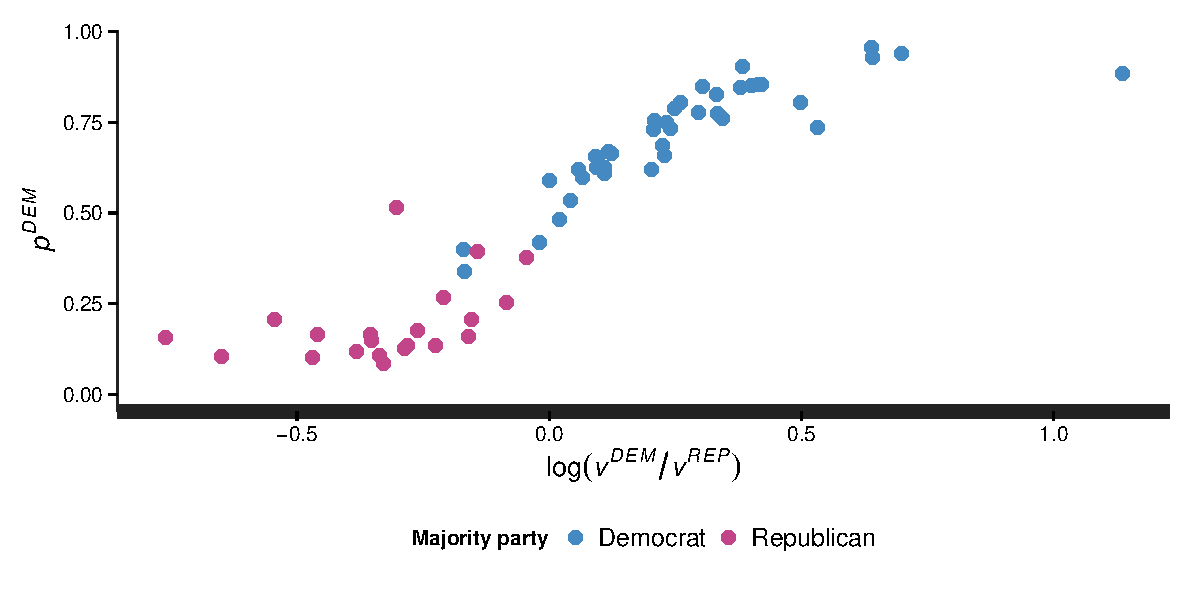
\includegraphics[scale=0.75]{sections/figs/logvratio_vs_pdem}
\caption{$\log{(v_t^{DEM} / v_t^{REP} )}$  vs. $p^{DEM}$}
\label{fig:log_vratio_vs_ptdem}
\end{figure}
%





%FIGURE
\begin{figure}
\centering
	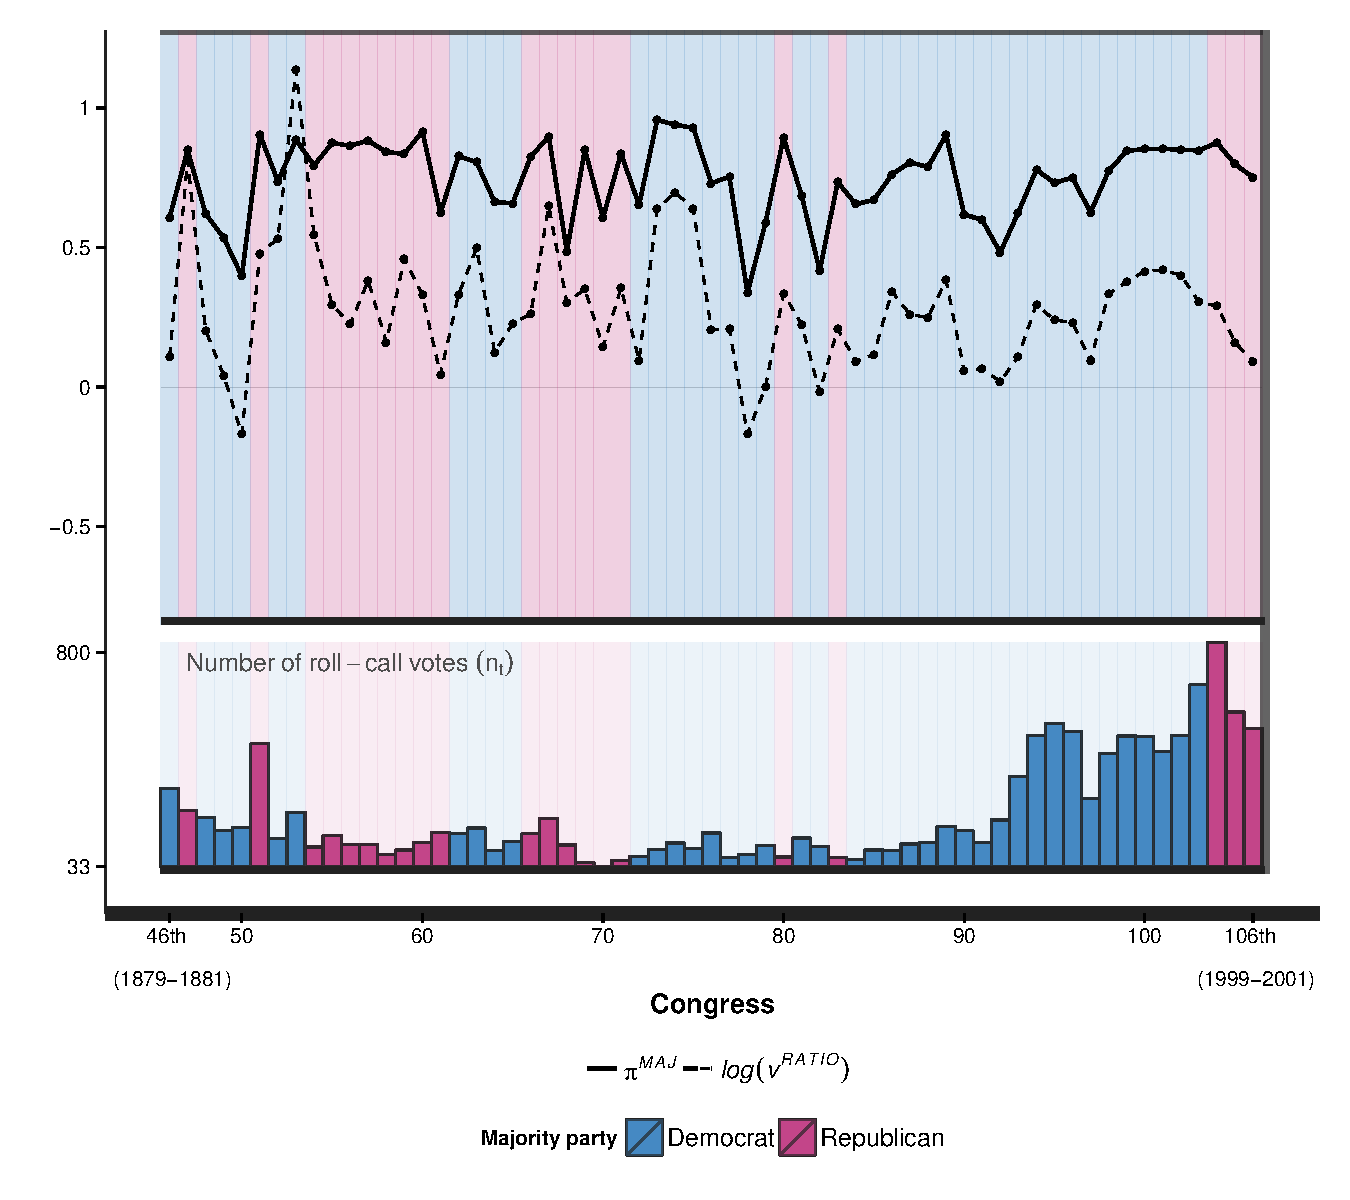
\includegraphics[scale=0.75]{sections/figs/vis_summary}
\caption{Visual summary of the data}
\label{fig:data_summary}
\end{figure}
%

One method of identifying bias toward or against the majority party is to estimate $E[p_t^{MAJ} |v_t^{MAJ}=0.5]$, the proportion of majority party victories conditional on equal vote share, and compare the estimate to $0.5$, the expected proportion of majority party victories in the absence of bias.  There are many close votes in the data -- that is, votes where $v_t^{MAJ} \approx 0$ -- which can be used to estimate $E[p_t^{MAJ} |v_t^{MAJ}=0.5]$.  Figure 2, below, shows the proportion of majority party victories under four different definitions of a close votes corresponding to margins of victory of 0.125\%, 0.25\%, 0.5\%, and 1.0\%. 

\vskip1cm
FIGURE
\vskip1cm

\section{Statistical and computational methods}
\subsection{Description of statistical model}
\label{subsection_methods}

\citeA{cox_gerrymandering_2007} propose two methods for checking their hypothesis of bias towards the majority party during the czar rule and post-packing eras. One strategy is to estimate separate models for four historical time periods of interest. \citeA{goodrich_designing_2012} point out that this ``imposes a particular periodization scheme that, while consistent with received wisdom, may or may not be the correct one" (p. 16). Cox and Katz's second approach is more promising in that it allows for greater parameter heterogeneity and makes fewer a priori assumptions about the underlying data generating process.\footnote{It is worth noting that making assumptions about the data generating process is in general not only unavoidable but also extremely important. The problem with the assumptions required for Cox and Katz's first method is not that they are implausible, but rather that periodization schemes per se are convenient abstractions that, in the context of quantitative historical analysis, can enforce a theoretically motivated but not empirically justified structure that should be learned rather than imposed.} However, as demonstrated below, there are other drawbacks to their design that can be overcome by following the guidelines for quantitative historical inquiry set forth in \citeA{wawro_designing_2014}. 

The analyses conducted by Cox and Katz concerns the estimation of parameters  $\lambda = (\lambda_t : t = 46, \dots, 106)$ representing bias (on the logit scale) toward the majority party in each $C_t$ (Congress $t$), which is done by maximum likelihood estimation of grouped logit models with linear predictor $ \lambda_t + \rho_t \log{\left(v_t^{RATIO} \right)}$. Here the parameter $\rho$ represents responsiveness, as defined above. 

The estimation of $\lambda$ and $\rho$ by grouped logit models follows naturally from solving the seats-votes equation for the average seat share, which in the legislative context of Cox and Katz's example is $p^{DEM}$, the expected roll-call win share for the Democrats 

{\singlespacing
$$  
  E(p^{DEM}_t)  = \left(1 + \exp{\left\{- \lambda_t - \rho_t \log{\left( v_t^{DEM}/v_t^{REP}  \right)}\right\}}\right)^{-1},
$$
}
%
\noindent which is the familiar logistic function. 

Cox and Katz's strategy is to estimate what they call ``a sort of running average" of bias across time (p. 116). To do this they take as their estimate of $\lambda_t$ the average estimate of $\lambda$ over the seven congresses centered at $t$, the set $\{C_\tau, t-3 \leq \tau \leq t+3\}$. However, this approach to modeling temporal dependence in $\lambda$ requires reusing the data to estimate models for each Congress (the observations for each Congress are used up to seven times).  \citeA{goodrich_designing_2012} point out that such recycling data can lead to overly precise parameter estimates. 

Although Cox and Katz do not acknowledge this potential for exaggerated precision, they do call attention to another important concern. To obtain reasonable estimates, their method requires a nontrivial amount of variation in average vote share between the seven Congresses that comprise each set $C_\tau$. 

The alternative analysis presented below overcomes both of these concerns by employing a hierarchical Bayesian framework with partial pooling. Following Cox and Katz, a BetaBinomial likelihood is used, however the linear predictor is replaced by the structured additive predictor $\eta$. The data model with logit link function is 

$$w_t^{MAJ} | n_t, \alpha_t, \beta_t \sim {\rm BetaBinomial}(n_t, \alpha_t, \beta_t),$$
$$ \alpha_t = \theta_t \phi, \qquad \beta_t = \theta_t (1 - \phi),$$
$$ \log\left({\frac{\theta_t}{1 - \theta_t}}\right) = \eta_t = f_{\lambda}(\lambda_t) + f_\rho \left(\log{(v_t^{RATIO})}\right).$$

The ${\rm BetaBinomial}(\alpha,\beta)$ distribution can be thought of as a compound distribution resulting from a binomial distribution where the probability parameter follows a ${\rm Beta}(\alpha,\beta)$ distribution. In other words, rather than assuming that the Congress-by-Congress probabilities of a majority party roll-call victory are independent and identically distributed -- in which case the binomial distribution would suffice -- the BetaBinomial  allows for direct modeling of the variation in the probability of victory through the Beta distribution. The parameters $\alpha$ and $\beta$ govern the shape of the Beta distribution, however it is both more intuitive and computationally attractive to reparameterize in terms of the mean $\theta$, which requires introducing a parameter $\phi$ as the sum of $\alpha$ and $\beta$.  This parameterization allows for ${\rm logit}(\theta)$ to be estimated by the semi-parametric structured additive predictor $\eta$ of the STAR model. 

Instead of Cox and Katz's ``sort of running average" approach, the hierarchical Bayesian STAR model entails estimating the unknown functions $f_\lambda$ and $f_\rho$. As we've seen, the vector of evaluations of the unknown functions can be conveniently expressed as the products 

{\singlespacing
$$
\mathbf{f}^{eval}_\lambda = \lambda \mathbf{M}_\lambda, 
\qquad 
\mathbf{f}^{eval}_\rho = \rho \mathbf{M}_\rho, 
$$
}
%
\noindent of the parameter vectors $\lambda$ and $\rho$ of length 61 (the number of Congresses in the data) and  $N \times 61$ design matrices  $\mathbf{M}_\lambda$ and  $\mathbf{M}_\rho$ (where $N$ is the total number of observations in the data). The predictor $\eta$ can be written compactly in vector notation as 

{\singlespacing
$$ \eta = f_\lambda(\lambda) +  f_\rho(\log{(v^{RATIO})}) = \lambda \mathbf{M}_\lambda + \rho \mathbf{M}_\rho.$$
}
%
\indent The matrices $\mathbf{M}_\lambda$ and $\mathbf{M}_\rho$ are identical in structure but not content. Since $\lambda$ plays the role of an intercept -- that is, the parameters in $\lambda$ are not coefficients -- the elements of $\mathbf{M}_\lambda$ are zeros and ones indicating the Congress to which each observation pertains. For $\mathbf{M}_\rho$ each element is either a zero or the appropriate value of $\log{(v^{RATIO})}$. 

% Discuss challenges with sparse matrices? Either here or in the lit review section

The priors for $f_{\lambda}$ and $f_{\rho}$ are expressed as distributions over the vectors $\lambda$ and $\rho$ as 
%
$$ 
p(\lambda | \tau_\lambda^2) \propto \exp{\left\{-\frac{1}{2\tau_\lambda^2} \: (\lambda - \bar{\lambda})^T \, \mathbf{P}  \, (\lambda - \bar{\lambda}) \right\}}, 
\qquad
p(\rho | \tau_\rho^2) \propto \exp{\left\{-\frac{1}{2\tau_\rho^2} \: (\rho - \bar{\rho})^T \, \mathbf{P} \, (\rho-\bar{\rho}) \right\}}
 $$

%
\noindent where the penalty matrix $\mathbf{P}$ encodes assumptions about the temporal dependence between Congresses. %
%\footnote{The impropriety of this prior stems from the fact that the matrix  $\mathbf{P}$ is not full rank.  The computational challenges this presents can be overcome by coding the model in a statistically equivalent but less intuitive form.} 
To model temporal dependence such that the set of Congresses $\partial_t = \{C_{t-2}, C_{t-1}, C_{t+1}, C_{t + 2} \}$ provides information about $C_t$, the undirected $RW_2$ prior discussed earlier is used to penalize deviations from this hypothesized trend. This corresponds to constructing $\mathbf{P}$ from the adjacency matrix $\mathbf{A}$ with $a_{ij} = 1$ if $C_j \in \partial_i$ and 0 otherwise.


%As alluded to above, modeling the temporal dependence between Congresses is accomplished via the choice of penalty matrix $\mathbf{P}$. To model temporal dependence such that the set of Congresses $\partial_t = \{C_{t-2}, C_{t-1}, C_{t+1}, C_{t + 2} \}$ provides information about $C_t$, an undirected form of a second order random walk or autoregressive prior is used to penalize deviations from this hypothesized trend. This corresponds to setting $\mathbf{P} = \mathbf{D} - \mathbf{A}$, where $\mathbf{A}$ is a symmetric matrix with $a_{ij} = 1$ if $C_j \in \partial_i$ and 0 otherwise, and $\mathbf{D}$ is a diagonal matrix such that $\forall i = j, \: d_{ij} = \sum_j a_{ij}$. It can be useful to conceptualize the neighbor relations described by each set $\partial_t$ as an undirected graph $G$ with vertices $V=\{C_t: t=46,\dots,106\}$ and edges connecting the vertices corresponding to neighboring Congresses.\footnote{Note that here the term ``neighbor" is not reserved only for adjacent Congresses, but rather any Congress in $\partial_t$ is considered a neighbor of Congress $t$.} The penalty matrix $\mathbf{P}$ then has a zero for each missing edge and the resulting multivariate normal distribution is a GMRF with respect to $G$.
%
%The matrices $\mathbf{A}$ and $\mathbf{D}$ are commonly referred to as the adjacency and degree matrices because encoded in $\mathbf{A}$ are all neighbor relationships (in this case a temporal relationship between Congresses) and the diagonal elements of $\mathbf{D}$ are the number of neighbors (the degree) of each vertex.
%
%To illustrate why this form of $\mathbf{P}$ captures these particular assumptions, consider $N$ measurements of a variable $x$, with each measurement made at one of $T$ evenly spaced points in time. For simplicity assume $N=T$ and that unit of $x$ is a unit of time.  The sequence of equally spaced time measurements $(x^{[t]})_{t=1}^T$ corresponds to a grid of points on a line.  Fahrmeir & Lang (2001) suggest several possible choices for a prior on a smooth function $f(x)$, the simplest of which is a first order random walk ($RW_1$) prior.  Under the $RW_1$ prior, the first differences
%
%$$\Delta_t = f(x^{[t]}) - f(x^{[t-1]})$$
%
%are treated as independent and identically distributed standard normal random variables. 
%
%While this formulation of the $RW_1$ prior is {\it directed}, conditioning also on $f(x^{[t+1]})$ -- one step into the future -- forms an undirected $RW_1$, where the neighbors of time $t$ are both $t-1$ and $t+1$.  The associated graph $G$ therefore has vertices $V=\{v_t : t=1,\dots,T\}$, each of which has two neighbors, with the exception of $v_1$ and $v_T$, which have one neighbor. The penalty matrix $\mathbf{P}$ corresponding to the $RW_1$ prior with equally with equally spaced observations is the tridiagonal matrix
%
%$$ \mathbf{P} = \mathbf{D} - \mathbf{A} =  \begin{bmatrix}
%1  	& -1 	& 		& 	& \\
%-1  	& 2 	& -1 		& 	& \\
%  	& -1 	& \ddots 	& \ddots	& \\
%  	&  	& \ddots 	& 2 	& -1\\
%  	&  	& 		& -1 	& 1\\
%\end{bmatrix}
%.
%$$
%
%The $RW_2$ prior used in this thesis is simply an extension of the $RW_1$ to the case where, in addition to $x^{[t-1]}$  and $x^{[t+1]}$, the measurements $x^{[t-2]}$  and $x^{[t+2]}$ are also considered neighbors of $x^{[t]}$. The construction of $\mathbf{P}$ as the matrix difference $\mathbf{D} - \mathbf{A}$ also allows the estimation of an optional scalar parameter $\gamma \in [0,1]$, which, as a coefficient on $\mathbf{A}$, can be interpreted as representing the strength of dependence (Rue and Held, 2005).\footnote{The resulting precision matrix $\mathbf{Q}= (\mathbf{D}- \gamma \mathbf{A})/\tau^2$ is the defining feature of the conditional autoregressive (CAR) model.  When $\gamma$ is fixed at 1, and thus $\mathbf{P}= \mathbf{D} - \mathbf{A}$, it is known as the intrinsic conditional autoregressive (ICAR) model.} In the results section it will be demonstrated that the degree to which the proposed model fits the data depends (slightly but non-negligibly) on the inclusion of $\gamma$. 



\subsection{Estimation using Stan}

For notational convenience, let $y$ denote the outcome $w^{MAJ}$ and $X$ denote the observed data $n$ and $v^{RATIO}$. We require the joint posterior distribution

{\singlespacing
\begin{align*}
p(\lambda, \rho, \tau^2_\lambda, \tau^2_\rho, \phi | y, X) & \propto p(\lambda, \rho, \tau^2_\lambda, \tau^2_\rho, \phi) p(y | \lambda, \rho, \tau^2_\lambda, \tau^2_\rho, \phi,  X)  \\
& = p(\phi) p(\tau^2_\lambda) p(\tau^2_\rho)  p(\lambda | \tau^2_\lambda) p(\rho | \tau^2_\rho) \prod_i p(y_i | \eta_i, X_i) 
\end{align*}
}
%
\noindent where the second line follows from assumptions of conditional independence.\footnote{In particular we assume that hyperparameters are mutually independent in their priors, $p(\lambda | \tau^2_\lambda)$ and $p(\rho | \tau^2_\rho)$ are conditionally independent, and the observations $y_i$ are independent conditional on parameters and predictors.}
%\footnote{The absence of the previously mentioned parameters $\alpha$, $\beta$, and $\theta$ from the expression for the posterior distribution is due to the fact that their values are determined by the other parameters.} 

Estimation is performed numerically by Markov chain Monte Carlo (MCMC) methods and implemented via RStan, the R interface to the probabilistic programming language and C++ library Stan \shortcite{rstan_software:2015}.\footnote{All relevant R and Stan code will be made publicly available in a repository on GitHub.} Although other existing software including BayesX, JAGS, and OpenBugs can sometimes be used to fit similar models, each has important limitations that Stan overcomes. Several of the many advantages to using Stan are discussed in the next section. Since there are no publicly available examples of fitting these models in Stan that we are aware of, the next section also provides a description of how the model is coded and estimated. 

\subsubsection{Brief introduction to Stan}

Stan is a probabilistic modeling language, MCMC sampler, and optimizer. The particular MCMC algorithm implemented in Stan is a variant of Hamiltonian Monte Carlo (HMC) called the no-U-turn sampler (NUTS) \shortcite{hoffman_2012}. Borrowing from physics the concepts and mathematics behind Hamiltonian dynamics, HMC treats the vector of unknown parameters as the position of a particle. In Hamiltonian dynamics, momentum and position change continuously over time, with the gradient of the particle's potential energy function --  which corresponds to the negative log posterior -- responsible for changes in momentum and momentum governing changes in position. Stan works by simulating a discretization of this process, making necessary corrections to preserve detailed balance (that is, to ensure that the resulting Markov chains are reversible). 

Several characteristics of HMC, and in particular Stan's implementation of HMC, make it a more appealing choice than traditional Metropolis-Hastings (M-H) and Gibbs samplers in many cases. Both M-H and Gibbs samplers suffer from random walk behavior that leads to inefficient exploration of the parameter space. Using gradient information, HMC can find posterior modes much more efficiently, greatly reducing the number of iterations required to obtain a sufficient number of effective draws from the posterior. 

M-H samplers in particular also require a great deal of tuning from the user. Although HMC itself does not overcome this problem, Stan automatically takes care of the tuning during a warmup period before sampling.\footnote{Users can also manually set tuning parameters, although this is rarely needed.} Gibbs sampling has an advantage over M-H in that it does not require tuning, but a serious drawback is that Gibbs sampling requires the full conditional distributions of all parameters. Except in a limited number of cases, full conditionals are difficult or impossible to derive, which results in a small number of prior distributions that are feasible to use with Gibbs samplers. In particular, conjugate priors are often used even when more believable priors are available. On the other hand, there is no advantage to conjugacy when using Stan. Users are free to specify priors that more accurately reflect their prior knowledge. For a more thorough introduction to Stan see \citeA{stan_development_team_stan_2015} and \citeA{gelman_bayesian_2013}.

\subsubsection{Data and transformed data}

\begin{figure}[h]
\begin{lstlisting}[language=Stan, frame=trBL]
data {
  // dimensions 
  int<lower=1>          N ; # number of observations 
  int<lower=1>          C ; # number of congresses (time periods)
  
  // arrays of variables 
  int<lower=1,upper=C>  cong[N] ;     # maps between obs & congress
  int<lower=1,upper=56> nVotes[N] ;   # number of votes
  int<lower=0,upper=55> nWins[N] ;    # number of maj party victories
  real                  lvRatio[N] ;  # log(vRatio)
  
  // inverse of penalty matrix 
  matrix[C,C]           Pinverse ; # for GMRF prior
}
\end{lstlisting}
\caption{Stan: {\tt data} block}
\label{stan_data}
\end{figure}

In the {\tt data} block of a Stan model (Figure~\ref{stan_data}) we declare the data that will be passed to Stan. The declarations below are all straightforward, except for the matrix {\tt Pinverse}, which is the inverse of the difference of the degree and adjacency matrices, which is precomputed and passed in as data. 

\begin{figure}[h]
\begin{lstlisting}[language=Stan, frame=trBL]
transformed data {
  real<lower=0> phi_scale ;     # scale for prior on phi
  real<lower=0> phi_loc ;       # location for prior on phi
  real<lower=0> tau_scale ;     # scale for priors on taus
  real<lower=0> tau_loc ;       # location for priors on taus
  matrix[C,C]   cholPinverse ;  # Cholesky decomposition 
  
  phi_loc <- 0 ;
  phi_scale <- 10 ;
  tau_loc <- 0 ;
  tau_scale <- 1 ;
  cholPinverse <- cholesky_decompose(Pinverse) ;
}
\end{lstlisting}
\caption{Stan: {\tt transformed data} block}
\label{stan_transformed_data}
\end{figure}


The {\tt transformed data} block (Figure~\ref{stan_transformed_data}) contains transformations of the variables declared in the {\tt data} block. In {\tt transformed data} the Cholesky decomposition of {\tt Pinverse} is computed; it will be used for a more efficient implementation of the multivariate normal distributions required for the GMRF priors. Values for the location and scale parameters of the Cauchy and normal distributions (to be used for priors) are also set in {\tt transformed data}. 






\subsubsection{Parameters and transformed parameters}

\begin{figure}[h]
\begin{lstlisting}[language=Stan, frame=trBL]
parameters {
  real          lambda_bar ;  # prior mean 
  real<lower=0> rho_bar ;     # prior mean 
  vector[C]     lambda ;      
  vector[C]     rho ;
  real<lower=0> phi_noise ;    
  real<lower=0> tau_sq_lambda ;  
  real<lower=0> tau_sq_rho ;
}
\end{lstlisting}
\caption{Stan: {\tt parameters} block}
\label{stan_parameters}
\end{figure}

In the {\tt parameters} and {\tt transformed parameters} blocks (Figures \ref{stan_parameters}, \ref{stan_transformed_parameters}) we declare model parameters and deterministic transformations of the declared parameters. 


%
\noindent Parameter names with the suffix ${\tt \_noise}$ denote variables to be given standard normal priors. Stan tends to work best if the target posterior distribution is marginally standard normal and uncorrelated and parameters on a  similar scale. This means that it can help improve efficiency and convergence if variables defined in {\tt parameters} are given standard normal priors when possible and then transformed in {\tt transformed parameters} to have the desired distribution.\footnote{This is an extremely oversimplified description and a thorough examination of the issue is beyond the scope of this thesis. See \citeA{betancourt_hamiltonian_2013} and \citeA{stan_development_team_stan_2015}.} 

\begin{figure}[h]
\begin{lstlisting}[language=Stan, frame=trBL]
transformed parameters {
  real<lower=0> phi ;
  
  // inverse CDF method, from standard normal to (half) Cauchy
  phi <- phi_loc + phi_scale * tan(pi()*(Phi_approx(phi_noise) - 0.5)) ;
}
\end{lstlisting}
\caption{Stan: {\tt transformed parameters} block}
\label{stan_transformed_parameters}
\end{figure}

In the {\tt transformed parameters} block, ${\tt phi\_noise}$ is transformed using the inverse-CDF method such that ${\tt phi}$ has a half-Cauchy distribution.\footnote{The inverse-CDF of the Cauchy distribution with location $\ell$ and scale $s$ is $F^{-1}(p, \ell,s)  = \ell + s \tan{\{ \pi (p - 0.5)\}}$. Thus if $z \sim \mathcal{N}(0,1)$ with CDF $\Phi$ then $\ell + s \tan{\{ \pi (\Phi(z) - 0.5)\}}$ is distributed Cauchy$(\ell, s)$. The transformation above therefore results in a half-Cauchy$({\tt phi\_loc}, {\tt phi\_scale})$ distribution due to the constraints that ${\tt phi\_noise}$ and ${\tt phi}$ be positive.}\footnote{The Cauchy prior can be considered weakly informative in that, while most of the mass is concentrated near the median, the tails are fat enough to allow for considerable variation. In fact, the variance of a Cauchy distribution is infinite.}



\subsubsection{Model}

In the {\tt model} block the likelihood and priors are specified. More precisely, Stan requires the log-likelihood and log-priors, the sum of which equals the log-posterior up to an additive constant.\footnote{Stan works on the log scale for the same reason as most other statistical software. Logarithms help avoid the loss of the numerical precision in addition to greatly simplifying expressions for complicated probability distributions.}
The priors include the standard normal on ${\tt phi\_noise}$ discussed above, normal priors for ${\tt lambda\_bar}$, ${\tt rho\_bar}$, ${\tt tau\_sq\_lambda}$, and ${\tt tau\_sq\_rho}$, and multivariate normal priors on ${\tt lambda}$ and ${\tt rho}$.\footnote{The function names in the {\tt model} block ending in ${\tt\_log}$ return the logarithm of the density function (e.g. ${\tt normal\_log(theta,0,1)}$ returns the logarithm of the normal density of ${\tt theta}$  with location 0 and scale 1). While Stan does support the familiar sampling statement notation (e.g. ${\tt theta \sim normal(0,1)}$), it is not used here because such notation is somewhat misleading. Using a sampling statement like ${\tt theta \sim normal(0,1)}$ does {\it not} mean that ${\tt theta}$ will be drawn from the standard normal distribution; it means that the logarithm of the standard normal density (up to a constant) evaluated at ${\tt theta}$ will be added to the total log probability accumulator. This can be expressed explicitly using the ${\tt increment\_log\_prob}$ and ${\tt normal\_log}$ functions; the statement ${\tt increment\_log\_prob(normal\_log(theta,0,1))}$ more accurately reflects Stan's execution under the hood. The only non-cosmetic difference between sampling statements and directly incrementing the log probability is that the former drops all constant terms. For a more detailed explanation see \citeA{stan_development_team_stan_2015}.} The Cholesky parameterization of the multivariate normal distribution is used for computational efficiency.\footnote{Instead of using {\tt multi\_normal\_cholesky} in the {\tt model} block, we could also specify the desired multivariate normal distribution in {\tt transformed parameters} by defining ${\tt lambda}$ (and analogously for ${\tt rho}$) to be  ${\tt lambda\_bar + (tau\_sq\_lambda * cholPinverse) * lambda\_noise}$, where ${\tt lambda\_noise}$ is a vector of iid standard normals. This follows from the fact that if $z$ is a $K$-vector of iid $N(0,1)$ variables and $\theta = \mu + L z$, where $LL' = \boldsymbol{\Sigma}$, then $\theta \sim \mathcal{N}_K (\mu, \boldsymbol{\Sigma})$. This is analogous to the univariate case where $\theta = \mu + \sigma z$ and $z \sim \mathcal{N}(0,1)$ implies that $\theta \sim \mathcal{N}(\mu, \sigma^2)$. Unlike the elements of $\theta$, the elements of $z$ are independent which can lead to large gains in efficiency for MCMC algorithms in terms of effective sample size \shortcite{stan_development_team_stan_2015}. This strategy did not end up being necessary for this model, but it is worth considering if effective sample sizes are low.} 

At the top of the {\tt model} block two vectors, {\tt alpha} and {\tt beta}, are also declared and will be filled in while looping over observations. This allows for the BetaBinomial likelihood to be vectorized for faster computation.

\begin{figure}
\begin{lstlisting}[language=Stan, frame=trBL]
model {
  // local/temporary variables
  real                logLik ;    # log likelihood
  real                logPrior ;  # log prior
  vector<lower=0>[N]  alphas ;    # shape1 for beta_binomial 
  vector<lower=0>[N]  betas ;     # shape2 for beta_binomial
  matrix[C,C]         L[2] ;      # cholesky of covmat
  
  L[1] <- diag_matrix(rep_vector(tau_sq_lambda,C)) * cholPinverse ;
  L[2] <- diag_matrix(rep_vector(tau_sq_rho,C)) * cholPinverse ;
  
  // priors
  logPrior <- (
    normal_log(lambda_bar, 0, 1) + 
    normal_log(rho_bar, 4, 2) + 
    normal_log(phi_noise, 0, 1) +
    normal_log(tau_sq_lambda, tau_loc, tau_scale) +
    normal_log(tau_sq_rho, tau_loc, tau_scale) +
    multi_normal_cholesky_log(lambda, rep_vector(lambda_bar,C), L[1]) +
    multi_normal_cholesky_log(rho, rep_vector(rho_bar,C), L[2]) 
  ) ;
  
  // likelihood
  for (n in 1:N) {
    real eta_n ;
    real theta_n ;
    eta_n <- lambda[cong[n]] + rho[cong[n]] * lvRatio[n] ;
    theta_n   <- inv_logit(eta_n) ;    
    alphas[n] <- theta_n * phi ;
    betas[n]  <- (1 - theta_n) * phi ;
  }
  // vectorized BetaBinomial
  logLik <- beta_binomial_log(nWins, nVotes, alphas, betas) ; 
  
  increment_log_prob(logPrior + logLik) ; 
}
\end{lstlisting}
\caption{Stan: {\tt model} block}
\label{stan_model}
\end{figure}
%
Expressing the likelihood in this way is perhaps less intuitive than incrementing the likelihood within the loop (and without creating the temporary {\tt alpha} and {\tt beta} variables)

\begin{lstlisting}[language=Stan, backgroundcolor=]
  logLik <- 0.0 ;
  for (n in 1:N) {
   ...
   logLik <- logLik +
   		beta_binomial_log(nWins[n], nVotes[n], 
   				  theta_n * phi, (1-theta_n) * phi) ;
  }
\end{lstlisting}
%
\noindent but filling in the elements of {\tt alpha} and {\tt beta} inside the loop and then using the vectorized version of the BetaBinomial is much faster. 

Note also that in the {\tt model} block the prior distributions are placed only on variables declared in {\tt parameters}  and not those defined in {\tt transformed parameters}. This is not a requirement, but assigning distributions to parameters declared in {\tt transformed parameters} requires the additional -- and potentially onerous -- step of accounting for changes in curvature due to the change of variables. For scalar parameters this entails calculating the log absolute derivative of the transform and incrementing the log probability by this value. For multivariate changes of variables the log probability must be incremented by the log absolute determinant of the corresponding Jacobian matrix.\footnote{This is explained in greater detail and with examples in \citeA{stan_development_team_stan_2015}. In brief, this adjustment is required to account for how the scale of the variable obtained by the transformation varies with respect to the original variable.}




\subsubsection{Generated quantities}

\begin{figure}[h]
\begin{lstlisting}[language=Stan, frame=trBL]
generated quantities {
  real        bias[C] ;  # bias toward majority party
  int         y_rep[N] ; # draws from posterior predictive distribution
  
  for (c in 1:C) 
    bias[c] <- inv_logit(lambda[c]) - 0.5 ;
  
  for (n in 1:N) {
    real eta_n ;
    real theta_n ;
    real alpha_n ;
    real beta_n ;
    eta_n <- lambda[cong[n]] + rho[cong[n]] * lvRatio[n] ;
    theta_n <- inv_logit(eta_n) ;    
    alpha_n <- phi * theta_n ;
    beta_n  <- phi * (1 - theta_n) ;
    // RNGs not vectorized in Stan so do it inside loop
    y_rep[n] <- beta_binomial_rng(nVotes[n], alpha_n, beta_n) ;
  }
}
\end{lstlisting}
\caption{Stan: {\tt generated quantities} block}
\label{stan_generated_quantities}
\end{figure}

The {\tt generated quantities} block allows for the computation of distributions of quantities of interest without affecting the log posterior specified in the model block. In this case we compute bias towards the majority party in each congress, which can be calculated as $-0.5$ plus the inverse-logit of the {\tt b\_bias} parameter. For model checking we also simulate data from the posterior predictive distribution, which is discussed in further detail below in \ref{subsection_model_checking}.\footnote{The random number generating functions are not currently vectorized in Stan, which is why the call to ${\tt beta\_binomial\_rng}$ is inside the loop in the {\tt generated quantities} block unlike the call to ${\tt beta\_binomial\_log}$ in the {\tt model} block.} 




\section{Results, convergence monitoring, and model checking}


\subsection{Results}
\label{subsection_results}

\begin{figure}
\centering
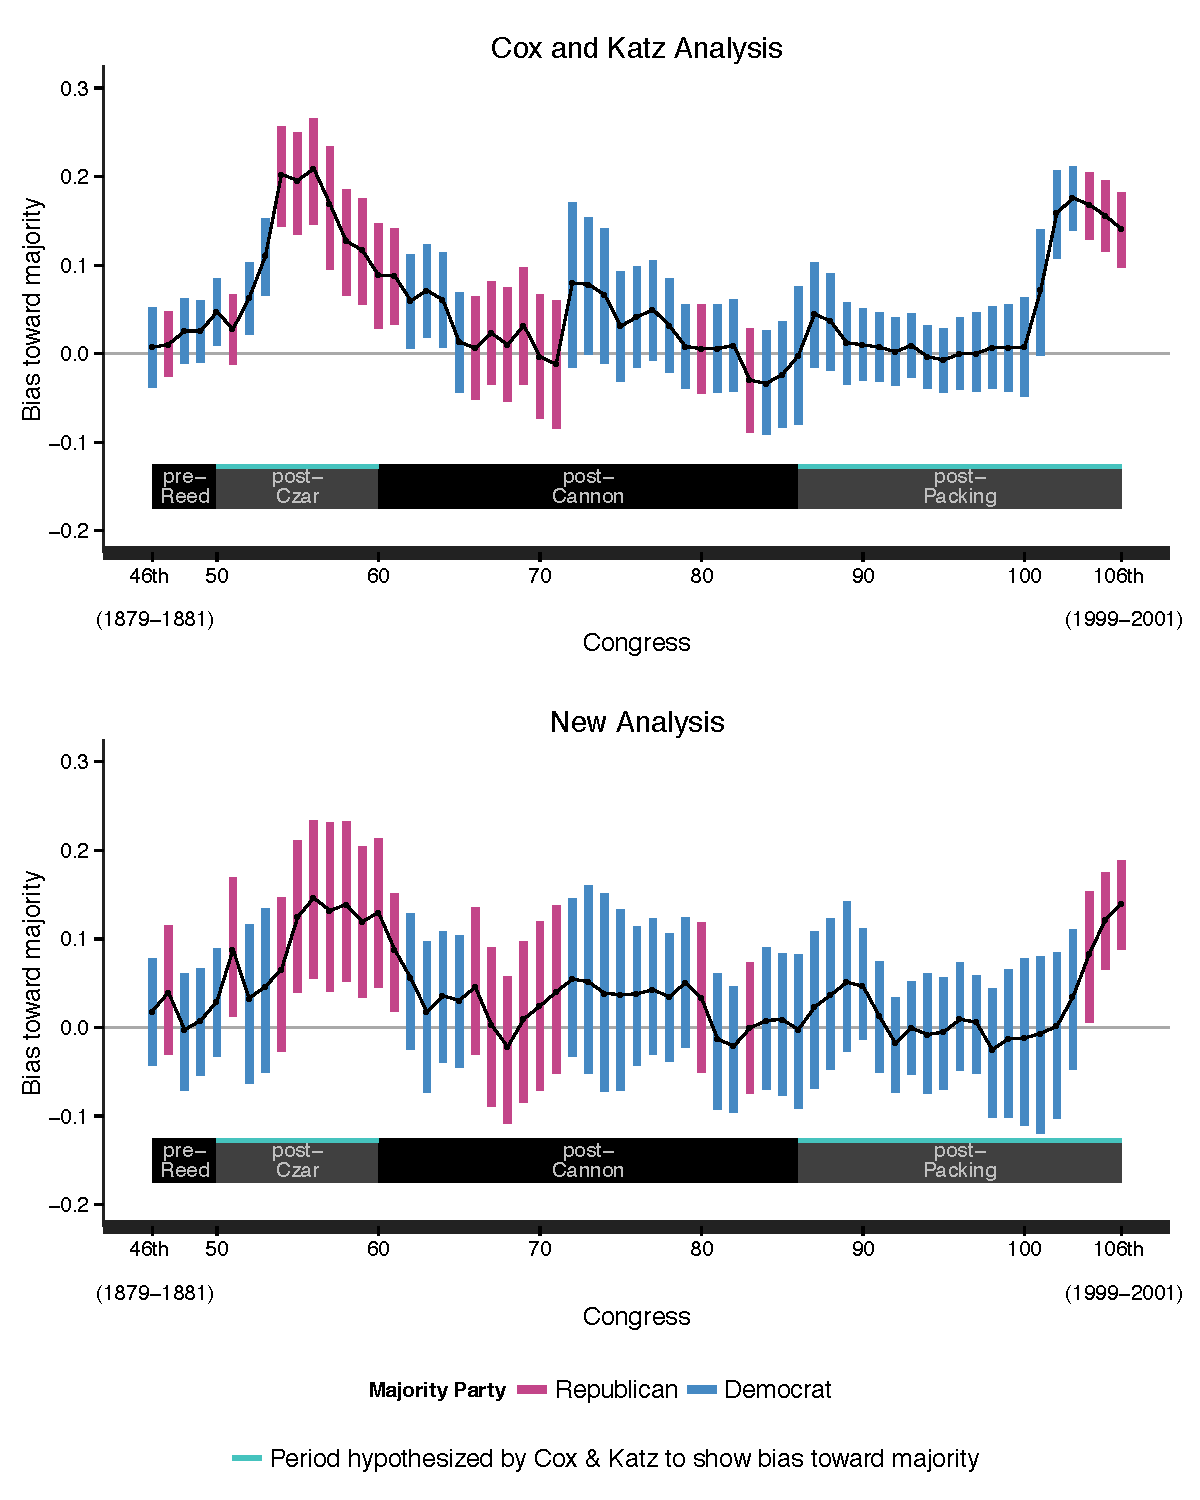
\includegraphics[scale=0.75]{sections/figs/ck_replication}
\caption{Estimated bias by Congress in Cox and Katz's analysis (top) and reanalysis (bottom). Vertical bars represent 95\%  intervals, with the black line connecting medians.}
\label{fig:ck_bias}
\end{figure}

Figure~\ref{fig:ck_bias} (p.~\pageref{fig:ck_bias}) shows the estimates of bias towards the majority party over time from Cox and Katz's analysis and the reanalysis conducted here. Immediately noticeable is the fact that the new estimates have greater uncertainties, which is to be expected due to the potential for Cox and Katz's method to produce overly precise estimates, as discussed in \ref{subsection_methods}. Furthermore, while the new results provide some support for the hypothesis of bias during the post-Czar and post-Packing periods, the evidence is much weaker than that found by Cox and Katz. 


\subsection{Convergence monitoring}
\label{subsection_convergence}



When inferences are made using posterior simulations generated by an MCMC algorithm it is essential to check for evidence of convergence to the target distribution. Although this process is not an exact science, there is no shortage of literature on the topic of monitoring convergence for MCMC and other iterative simulation algorithms. The various convergence diagnostics used below are introduced informally. Formal definitions, computational details and recommended best practices can be found in \citeA{gelman_handbook_2011}, \citeA{gelman_bayesian_2013}, and \citeA{stan_development_team_stan_2015}.

Eight randomly initialized chains of 1000 iterations (including 500 discarded warmup iterations) were simulated.\footnote{People new to HMC, NUTS, and Stan are often surprised by how few iterations are typically required, as it is not uncommon for Gibbs (and poorly tuned M-H) samplers to require hundreds of thousands of iterations to achieve convergence.} The distributions of three diagnostics calculated from the posterior sample are shown in Figure~\ref{fig:ck_diagnostics}. 

\begin{figure}[h]
\centering
	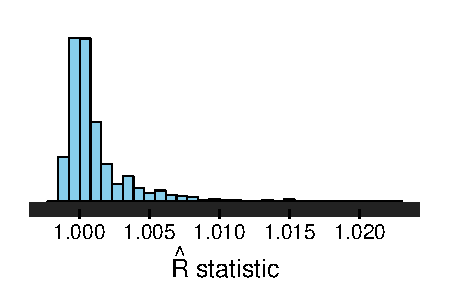
\includegraphics[scale=0.7]{sections/figs/rhat}
	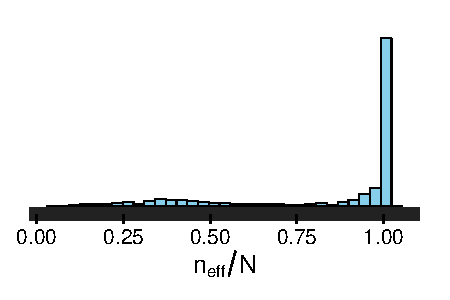
\includegraphics[scale=0.7]{sections/figs/neff}
	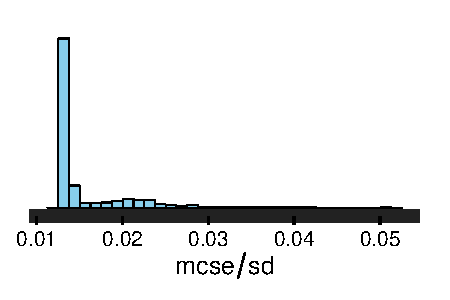
\includegraphics[scale=0.7]{sections/figs/mcse}
\caption{Distributions of diagnostics computed from the MCMC draws. From left to right: \newline ({\bf a}) Potential scale reduction factor $\hat{R}$ \newline ({\bf b}) Ratio of effective sample size to total sample size ($n_{\it eff}/N$) \newline ({\bf c}) Ratio of Monte Carlo error to posterior standard deviation ($mcse/sd$)}
\label{fig:ck_diagnostics}
\end{figure}

Figure~{\ref{fig:ck_diagnostics}a} shows the distribution of the estimates of the potential scale reduction statistic $\hat{R}$  \shortcite{gelman_rhat_1992}. The $\hat{R}$ statistic is a comparison of the variance of the simulations within individual chains to that of the simulations when chains are pooled. Here, the distribution of $\hat{R}$ shows that for all parameters the value is approximately one, indicating that little would be gained by running longer chains \shortcite{gelman_handbook_2011}. 

Figure~{\ref{fig:ck_diagnostics}b} shows the distribution of the ratio of effective sample size to the number of iterations ($n_{\it eff}/N$). Roughly speaking, $n_{\it eff}$ is an estimate of the number of {\it independent} draws from the posterior distribution that would have the same expected variance as the $N$ {\it dependent} draws actually obtained from the Markov chains. In this case $n_{\it eff}/N$ for all parameters is close to the ideal value of one, a reflection of Stan's efficiency. 


Figure~{\ref{fig:ck_diagnostics}c} shows the distribution of the ratio of Monte Carlo error to the estimated standard deviation ($mcse/sd$). Monte Carlo error is a measure of imprecision due to approximating the posterior distribution by the MCMC simulations. As the number of iterations increases $mcse$ goes to zero and the standard deviation of the draws converges to the posterior standard deviation. The distribution in Figure~\ref{fig:ck_diagnostics} shows that for all parameters the relative error $mcse/sd$ is less than five percent, which, for the inferential goals of this analysis is negligible. For instance, Figure~\ref{fig:ck_example_posterior} shows the estimated posterior density for the parameter corresponding to bias towards the majority party in the 79th congress.\footnote{There is nothing special about the 79th congress for this purpose. A single congress was chosen at random to use as an example.} 
%
\begin{figure}[h]
\centering
	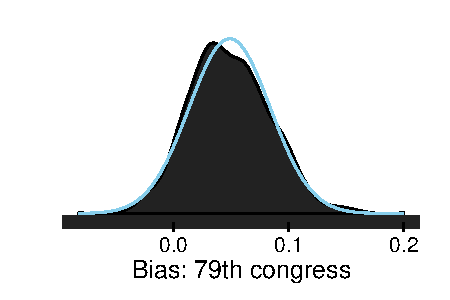
\includegraphics[scale=0.75]{sections/figs/example_posterior}
\caption{Posterior kernel density estimate for bias towards the majority party in the 79th congress. Normal density curve in blue.}
\label{fig:ck_example_posterior}
\end{figure}
%
\noindent The posterior is approximately normal, with mean and standard deviation estimates of roughly $0.054$ and $0.0368$, respectively. The estimated $mcse$ is $0.0007$, which is inconsequential when compared to the uncertainty about the parameter in the posterior distribution.   


Trace plots for all parameters were also examined as well as additional quantities specific to HMC and NUTS.\footnote{For example, checking that the tree depth used by NUTS is well below the user-specified maximum, ensuring that there are no post-warmup leapfrog iterations with diverging error, etc.}




\subsection{Model checking}
\label{subsection_model_checking}

% Should probably do pp checks after aggregating over the sub periods for each congress.  

\begin{figure}
\centering
	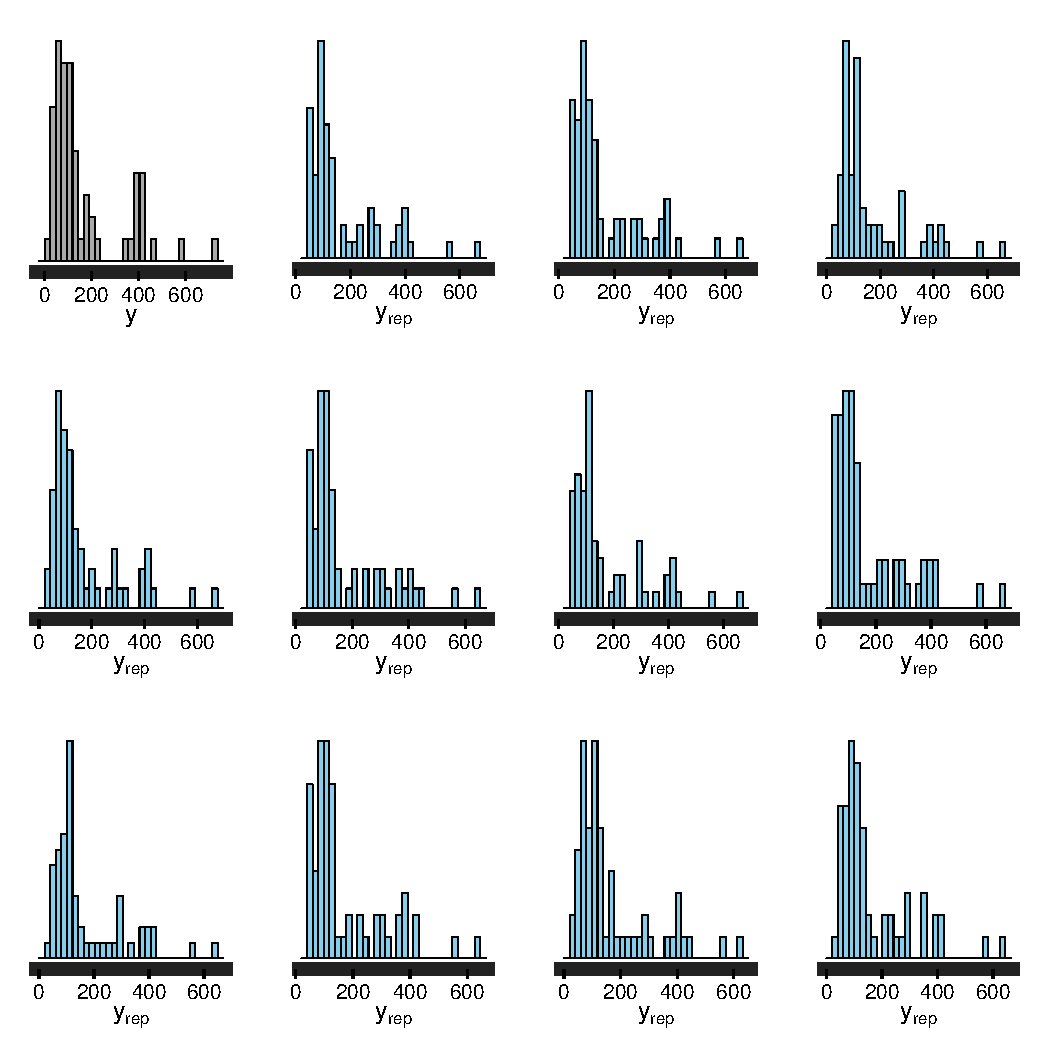
\includegraphics[scale=0.7]{sections/figs/ck_pp_y_vs_yrep_hists}
\caption{Replications from posterior predictive distribution vs. observed data}
\label{fig:ck_pp_hists}
\end{figure}

\begin{figure}
\centering
	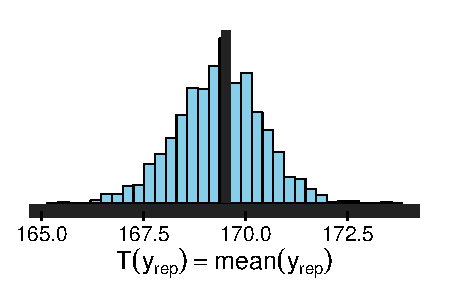
\includegraphics[scale=0.75]{sections/figs/test_stats_mean}
	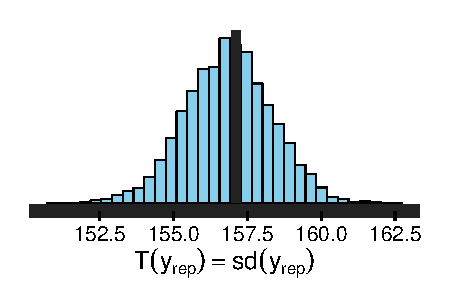
\includegraphics[scale=0.75]{sections/figs/test_stats_sd}
\caption{Distributions of test statistics $T(y_{rep})$. The vertical bar is the observed value $T(y)$.}
\label{fig:ck_pp_test_statistics}
\end{figure}

\begin{figure}
\centering
	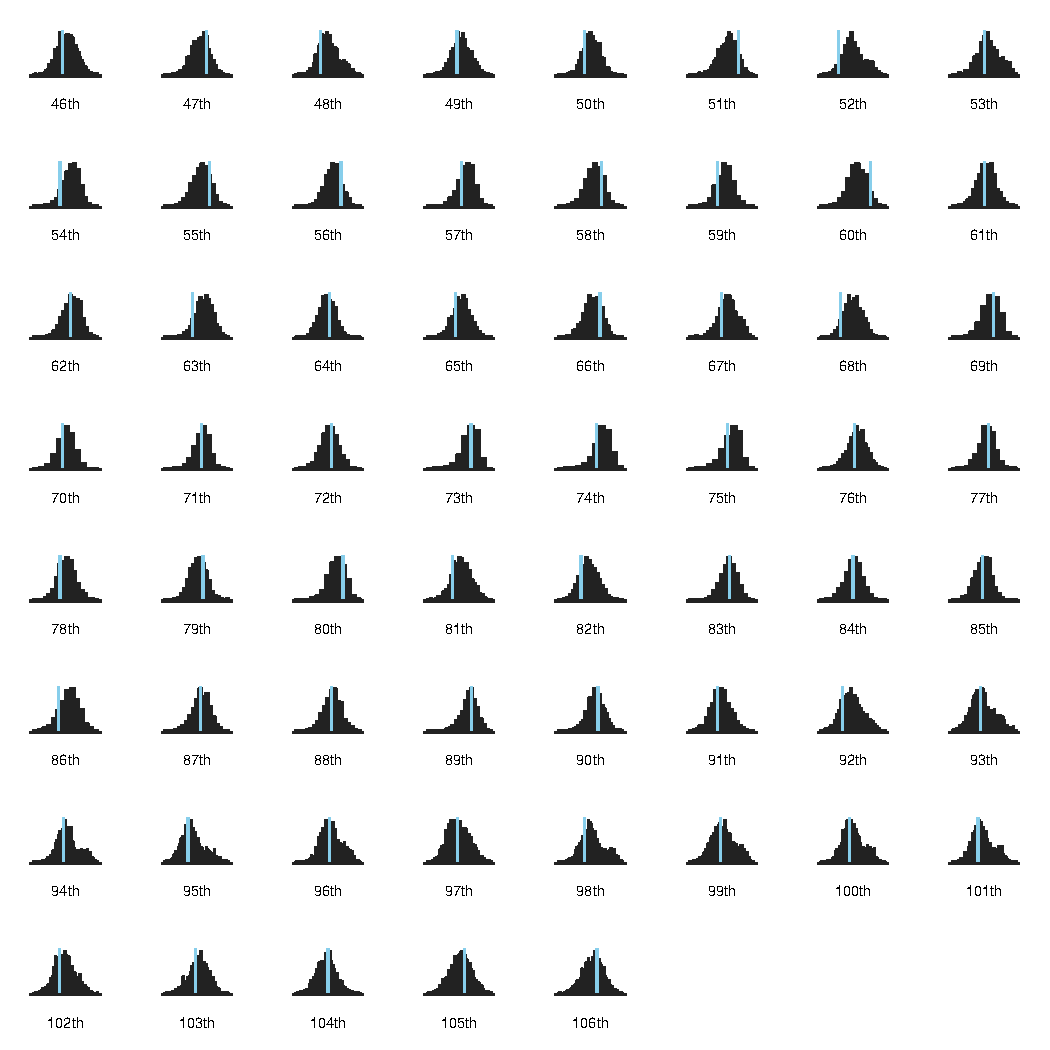
\includegraphics[scale=0.8]{sections/figs/ck_pp_nWins_hists}
\caption{Random sample of replicated data sets from posterior predictive distribution $p(y^{\it rep} | y)$ vs. observed data $y$ (vertical line) by Congress.}
\label{fig:ck_pp_nWins_hists}
\end{figure}




%\chapter{Farhang and Katznelson}

To illustrate the utility of STAR models, Wawro and Katznelson (2013) conduct a reanalysis of Farhang and Katznelson (2005). Farhang and Katznelson argue that drastic changes in the Democratic party's position on labor-friendly policies occurred during the time period of time between New Deal and Fair Deal, largely due to a growing divide between norther and southern Democrats. 

In this section we expand on the reanalysis proposed by Wawro and Katznelson. 

% Something about how this analysis includes time and space as opposed to cox and katz which is just time

\section{Data} 

The data used by Farhang and Katznelson pertains to roll-call votes in the 73rd through 80th Congresses (1933--1948). The outcome of interest is a binary variable indicating whether a senator $s$ from region $r$ voted in favor of the prolabor position on roll-call vote $v$ in Congress $t$

$$L_{srtv} = 
\begin{cases}
1, & \text{ if senator $s$ from region $r$ votes prolabor on vote $v$ at time $t$} \\
0, & \text{ otherwise.}
\end{cases}
$$

The possible values for region are Non-South (NS), Border South (BS), and Deep South (DS). 

Predictors include the proportion of African Americans living in the senator's home region $(AA)$, the proportion of individual's in the senator's home region living in urban areas ($URB$), a measure of unionization 
%\footnote{Include description from W\&K paper}
$(UN)$, and indicators for Democratic party membership $(DEM)$ and membership on the committee charged with overseeing labor-related issues $(COM)$.  % this is maybe too close to the wording in W&K

% say something about why these variables are relevant

% FIGURES summarizing data % 

\section{Method of analysis}

\subsection{The map as an undirected graph}

Unlike in the Cox and Katz analysis, here we want to account for variation and dependence over both temporal and spatial dimensions. From the three regions and eight congresses in the data we construct the $3 \times 8$ map with cells $c_1,c_2, \dots, c_{24}$ shown in Table~\ref{table:map_degree}. The value displayed in cell $c_{j}$ is the number of cells considered neighbors of $c_{j}$

$$ c_{j} = \sum_{k = 1}^{24} \textit{Ne}(j,k),$$

\noindent where the neighbor function $\textit{Ne}(j,k)$ is 1 if $c_j$ and $c_k$ are neighbors and $0$ otherwise. The value of each $c_j$ is determined by our subjective choice of the form of the neighbor function, which should be informed by a substantive theory about the temporal and spatial dependence. 

The values in Table~\ref{table:map_degree} correspond to using an undirected neighbor function that considers adjacency to be vertical, horizontal and diagonal. For example, this form of the neighbor function allows for dependence between the Border South region in the 76th Congress and the Non-South region in the 77th Congress. Other possible neighbor functions might only allow for dependence across regions in the same time period, or only allow dependence on prior time periods, or allow dependence on time periods even further into the past or future.    

%\begin{table}[ht]
%\centering
%\begin{tabular}{l|rrrrrrrr}
%\textbf{Region}/\textbf{Congress} & 73rd & 74th & 75th & 76th & 77th & 78th & 79th & 80th \\ 
%  \toprule
%Non-South &   1 &   4 &   7 &  10 &  13 &  16 &  19 &  22 \\ 
%  Border South &   2 &   5 &   8 &  11 &  14 &  17 &  20 &  23 \\ 
%  Deep South &   3 &   6 &   9 &  12 &  15 &  18 &  21 &  24 \\ 
%   \bottomrule
%\end{tabular}
%\caption{\small The $3 \times 8$ map assigning a unique identifier for each region/Congress pair}
%\label{table:map_id}
%\end{table}


\begin{table}[ht]
\centering
\begin{tabular}{l|rrrrrrrr}
\textbf{Region}/\textbf{Congress} & 73rd & 74th & 75th & 76th & 77th & 78th & 79th & 80th \\ 
 \toprule
Non-South 	
& $3_{(1)}$ & $5_{(4)}$ & $5_{(7)}$ & $5_{(10)}$ & $5_{(13)}$ & $5_{(16)}$ & $5_{(19)}$ & $3_{(22)}$ \\ 
Border South 	
& $5_{(2)}$ & $8_{(5)}$ & $8_{(8)}$ & $8_{(11)}$ & $8_{(14)}$ & $8_{(17)}$ & $8_{(20)}$ & $5_{(23)}$ \\ 
Deep South 	
& $3_{(3)}$ & $5_{(6)}$ & $5_{(9)}$ & $5_{(12)}$ & $5_{(15)}$ & $5_{(18)}$ & $5_{(21)}$ & $3_{(24)}$ \\ 
   \bottomrule
\end{tabular}
\caption{\small The $3 \times 8$ map where the cell contents are the number of neighbors. The subscripts assign each region/Congress pair a unique identifier from 1 to 24. Adjacency is vertical, horizontal, and diagonal.}
\label{table:map_degree}
\end{table}


Using the indices $r \in \{1,\dots, R\}$ (where in this case $R = 24$) from Table~\ref{table:map_degree}, we can 
reconceptualize the map as an undirected graph with $R$ vertices and with edges connecting neighbors. We can then make the two $R \times R$ matrices -- the symmetric adjacency matrix and diagonal degree matrix -- needed for constructing the precision matrix for the GMRF prior. 


%\clearpage
%
%\subsection{Notation}
%
%\begin{tabular}{ll}
%$N \approx 8000$ & Number of observations in the data. \\[5pt]
%
%$R = 24$ & Number of groups (i.e. region/period combos).  \\[5pt]
%
%$\textsc{urb}$, $\textsc{aa}$, $\textsc{un}$ & The three $N \times 1$ vectors for {\tt urbanpct}, {\tt aapct}, and {\tt unionpop} variables. \\[5pt]
%
%$\mathbf{M}$ & $N \times R$ matrix with $m_{ij} = 1$ if obs $i$ is from region-period $j$, and 0 otherwise. \\[5pt]
%
%$\mathbf{X}_1, \mathbf{X}_2, \mathbf{X}_3$ & $N \times R$ matrices with $x_{ij} =$ $i$th value of 
% \textsc{urb} (for $\mathbf{X}_1$), \textsc{aa} (for $\mathbf{X}_2$), \\
% 
% & or \textsc{un} (for $\mathbf{X}_3$) if obs $i$ is from region-period $j$, and 0 otherwise. \\[5pt]
%
%$\mathbf{Z} $ & $N \times 2$ matrix with party and committee indicators.  \\[5pt]
%
%$y$ & $N \times 1$ vector containing the indicator for pro-labor vote. 
%
%\end{tabular}



\vskip1in
\subsection{Model}

Conditional on parameters $\theta$, the observations of the binary indicator $L$ are assumed to be independent and follow a Bernoulli distribution. Here, the structured additive predictor $\eta = {\rm logit}(\theta)$ is 

$$\log{\left(\frac{\theta_{srtv}}{1 - \theta_{srtv}}\right)} = \eta_{srvt} = \alpha_0 + f_1 (\alpha_{rt}) + f_2 (UN_{srt}) + f_3 (URB_{srt}) + f4(AA_{srt}) + u_{srt}' \gamma, $$

\noindent where $\alpha_0$ represents a global intercept, $\alpha_{rt}$ is the region-period specific deviation from $\alpha_0$, and $\mathbf{u}$ includes $DEM$ and $COM$, predictors with effects assumed not to vary across region and time period.
 
As in the Cox and Katz model, we can express the vector of evaluations of each unknown function $f_j$ as the product of a design matrix $\mathbf{M}_j$ and a parameter vector, here denoted $\beta_j$. We can then write the structured additive predictor $\eta$ in matrix form as 
 
$$\eta = \mathbf{u}\gamma + \alpha_0 + \left( \sum_{j=1}^{4} \mathbf{M}_j \beta_j \right). $$
 
Specifying GMRF smoothness priors over regions and periods corresponds to the zero-mean multivariate normal priors

$$ p(\beta_j | \tau^2_j) \propto  \exp{\left(-\frac{1}{2\tau_j^2} \beta_j^T \mathbf{P}^{-1} \beta_j \right)}. $$

Weakly informative Gaussian priors are used for the coefficients $\gamma$. Prior distributions for the global intercept $\alpha_0$ and the hyperparameters $\tau_j$ are discussed below in the Estimation section. 








%For $j = 1, \dots, J$ the precision matrix $\mathbf{K}_j$ is defined as $\mathbf{K}_j = \tau_j \left(\mathbf{D} - \rho_j \mathbf{A}\right).$ The matrices $\mathbf{A}$ and $\mathbf{D}$ are the symmetric adjacency matrix and diagonal degree matrix. 
%
%\vskip 1cm
%
%For each precision matrix $\mathbf{K}_{R \times R}$, we can interpret its elements as follows:
%
%\begin{itemize}
%\item For $i \neq j$, element $k_{ij}$ is conditional covariance between $i$ and $j$, given all the variables except $i$ and $j$, except the sign of the conditional covariance is flipped.
%
%\item For $i = j$, element $K_{ij}$ is the conditional variance of $i$, given all the variables except $i$.
%\end{itemize}
%
%This enables us to go from the full-conditional relationships that GeoBUGS utilizes for Gibbs sampling to the joint form that Stan needs for HMC. \\
%
%


%\subsection{Hyperpriors}
%
%Let $\lambda_j \sim {\rm Exponential}(1)$ and let $\tau_j = \bar{\tau}\lambda_j $, which implies
%
%$$\tau_j \sim {\rm Exponential}(1/\bar{\tau}), $$
%
%where $\bar{\tau} > 0$ is the common mean for the $\tau_j$'s. Give $\bar{\tau}$ an improper flat prior over $\mathbb{R}^+.$ \\
%
%
%
%
%\noindent Let $\rho_j \sim {\rm Beta}(s_1, s_2)$, where $s_1 = \gamma \bar{\rho}$,  and $s_2 = \gamma(1-\bar{\rho})$, where $\gamma$ is either an estimated positive dispersion parameter or fixed (e.g. $\gamma = 1$). For the common mean $\bar{\rho} \in (0,1)$ let $\bar{\rho} \sim {\rm Unif}(0,1)$.    \\







%
%\begin{table}[ht]
%\scriptsize
%\centering
%$$  \begin{array}{r|rrrrrrrrrrrrrrrrrrrrrrrr} 
%  & 1 & 2 & 3 & 4 & 5 & 6 & 7 & 8 & 9 & 10 & 11 & 12 & 13 & 14 & 15 & 16 & 17 & 18 & 19 & 20 & 21 & 22 & 23 & 24 \\ 
%\midrule
%1 & 3 & \!-1\! & 0 & \!-1\! & \!-1\! & 0 & 0 & 0 & 0 & 0 & 0 & 0 & 0 & 0 & 0 & 0 & 0 & 0 & 0 & 0 & 0 & 0 & 0 & 0 \\ 
%  2 & \!-1\! & 5 & \!-1\! & \!-1\! & \!-1\! & \!-1\! & 0 & 0 & 0 & 0 & 0 & 0 & 0 & 0 & 0 & 0 & 0 & 0 & 0 & 0 & 0 & 0 & 0 & 0 \\ 
%  3 & 0 & \!-1\! & 3 & 0 & \!-1\! & \!-1\! & 0 & 0 & 0 & 0 & 0 & 0 & 0 & 0 & 0 & 0 & 0 & 0 & 0 & 0 & 0 & 0 & 0 & 0 \\ 
%  4 & \!-1\! & \!-1\! & 0 & 5 & \!-1\! & 0 & \!-1\! & \!-1\! & 0 & 0 & 0 & 0 & 0 & 0 & 0 & 0 & 0 & 0 & 0 & 0 & 0 & 0 & 0 & 0 \\ 
%  5 & \!-1\! & \!-1\! & \!-1\! & \!-1\! & 8 & \!-1\! & \!-1\! & \!-1\! & \!-1\! & 0 & 0 & 0 & 0 & 0 & 0 & 0 & 0 & 0 & 0 & 0 & 0 & 0 & 0 & 0 \\ 
%  6 & 0 & \!-1\! & \!-1\! & 0 & \!-1\! & 5 & 0 & \!-1\! & \!-1\! & 0 & 0 & 0 & 0 & 0 & 0 & 0 & 0 & 0 & 0 & 0 & 0 & 0 & 0 & 0 \\ 
%  7 & 0 & 0 & 0 & \!-1\! & \!-1\! & 0 & 5 & \!-1\! & 0 & \!-1\! & \!-1\! & 0 & 0 & 0 & 0 & 0 & 0 & 0 & 0 & 0 & 0 & 0 & 0 & 0 \\ 
%  8 & 0 & 0 & 0 & \!-1\! & \!-1\! & \!-1\! & \!-1\! & 8 & \!-1\! & \!-1\! & \!-1\! & \!-1\! & 0 & 0 & 0 & 0 & 0 & 0 & 0 & 0 & 0 & 0 & 0 & 0 \\ 
%  9 & 0 & 0 & 0 & 0 & \!-1\! & \!-1\! & 0 & \!-1\! & 5 & 0 & \!-1\! & \!-1\! & 0 & 0 & 0 & 0 & 0 & 0 & 0 & 0 & 0 & 0 & 0 & 0 \\ 
%  10 & 0 & 0 & 0 & 0 & 0 & 0 & \!-1\! & \!-1\! & 0 & 5 & \!-1\! & 0 & \!-1\! & \!-1\! & 0 & 0 & 0 & 0 & 0 & 0 & 0 & 0 & 0 & 0 \\ 
%  11 & 0 & 0 & 0 & 0 & 0 & 0 & \!-1\! & \!-1\! & \!-1\! & \!-1\! & 8 & \!-1\! & \!-1\! & \!-1\! & \!-1\! & 0 & 0 & 0 & 0 & 0 & 0 & 0 & 0 & 0 \\ 
%  12 & 0 & 0 & 0 & 0 & 0 & 0 & 0 & \!-1\! & \!-1\! & 0 & \!-1\! & 5 & 0 & \!-1\! & \!-1\! & 0 & 0 & 0 & 0 & 0 & 0 & 0 & 0 & 0 \\ 
%  13 & 0 & 0 & 0 & 0 & 0 & 0 & 0 & 0 & 0 & \!-1\! & \!-1\! & 0 & 5 & \!-1\! & 0 & \!-1\! & \!-1\! & 0 & 0 & 0 & 0 & 0 & 0 & 0 \\ 
%  14 & 0 & 0 & 0 & 0 & 0 & 0 & 0 & 0 & 0 & \!-1\! & \!-1\! & \!-1\! & \!-1\! & 8 & \!-1\! & \!-1\! & \!-1\! & \!-1\! & 0 & 0 & 0 & 0 & 0 & 0 \\ 
%  15 & 0 & 0 & 0 & 0 & 0 & 0 & 0 & 0 & 0 & 0 & \!-1\! & \!-1\! & 0 & \!-1\! & 5 & 0 & \!-1\! & \!-1\! & 0 & 0 & 0 & 0 & 0 & 0 \\ 
%  16 & 0 & 0 & 0 & 0 & 0 & 0 & 0 & 0 & 0 & 0 & 0 & 0 & \!-1\! & \!-1\! & 0 & 5 & \!-1\! & 0 & \!-1\! & \!-1\! & 0 & 0 & 0 & 0 \\ 
%  17 & 0 & 0 & 0 & 0 & 0 & 0 & 0 & 0 & 0 & 0 & 0 & 0 & \!-1\! & \!-1\! & \!-1\! & \!-1\! & 8 & \!-1\! & \!-1\! & \!-1\! & \!-1\! & 0 & 0 & 0 \\ 
%  18 & 0 & 0 & 0 & 0 & 0 & 0 & 0 & 0 & 0 & 0 & 0 & 0 & 0 & \!-1\! & \!-1\! & 0 & \!-1\! & 5 & 0 & \!-1\! & \!-1\! & 0 & 0 & 0 \\ 
%  19 & 0 & 0 & 0 & 0 & 0 & 0 & 0 & 0 & 0 & 0 & 0 & 0 & 0 & 0 & 0 & \!-1\! & \!-1\! & 0 & 5 & \!-1\! & 0 & \!-1\! & \!-1\! & 0 \\ 
%  20 & 0 & 0 & 0 & 0 & 0 & 0 & 0 & 0 & 0 & 0 & 0 & 0 & 0 & 0 & 0 & \!-1\! & \!-1\! & \!-1\! & \!-1\! & 8 & \!-1\! & \!-1\! & \!-1\! & \!-1\! \\ 
%  21 & 0 & 0 & 0 & 0 & 0 & 0 & 0 & 0 & 0 & 0 & 0 & 0 & 0 & 0 & 0 & 0 & \!-1\! & \!-1\! & 0 & \!-1\! & 5 & 0 & \!-1\! & \!-1\! \\ 
%  22 & 0 & 0 & 0 & 0 & 0 & 0 & 0 & 0 & 0 & 0 & 0 & 0 & 0 & 0 & 0 & 0 & 0 & 0 & \!-1\! & \!-1\! & 0 & 3 & \!-1\! & 0 \\ 
%  23 & 0 & 0 & 0 & 0 & 0 & 0 & 0 & 0 & 0 & 0 & 0 & 0 & 0 & 0 & 0 & 0 & 0 & 0 & \!-1\! & \!-1\! & \!-1\! & \!-1\! & 5 & \!-1\! \\ 
%  24 & 0 & 0 & 0 & 0 & 0 & 0 & 0 & 0 & 0 & 0 & 0 & 0 & 0 & 0 & 0 & 0 & 0 & 0 & 0 & \!-1\! & \!-1\! & 0 & \!-1\! & 3 \\ 
%\end{array} $$
%\caption{The ``Laplacian matrix" $\mathbf{L} = \mathbf{D} - \mathbf{A}$. The precision matrix $\mathbf{K}_j$ is $\mathbf{K}_j = \tau_j (\mathbf{D} - \rho_j \mathbf{A})$, where $\tau_j  > 0$ and $\rho_j \in (0,1)$. Thus $\rho_j \to 1 \implies \mathbf{K}_j \to \tau_j \mathbf{L}$.}
%\end{table}





\pagebreak
\nocite{r_software}
\singlespacing
\bibliography{bibliography.bib}

\end{document}